\section{Pendahuluan}
\subsection{Latar Belakang}
Pada modul kedua ini, kita akan membahas perbandingan hasil (ADC) analog to digital converter pada Arduino dan Osiloskop.Analog to Digital Converter (ADC) adalah perangkat yang berfungsi untuk mengubah sinyal analog menjadi sinyal digital. 
Sinyal analog adalah sinyal yang memiliki nilai yang berubah-ubah dalam waktu, sedangkan sinyal digital adalah sinyal yang memiliki nilai yang berubah-ubah dalam waktu tetapi hanya memiliki dua nilai, yaitu 0 dan 1.
\\\\
ADC umumnya menggunakan metode Successive Approximation Register (SAR) atau metode lainnya untuk mengkonversi sinyal analog menjadi sinyal digital. 
Misalnya, pada Arduino, ADC menggunakan metode SAR untuk mengkonversi tegangan analog menjadi nilai digital yang dapat diproses oleh mikrokontroler.
\\\\
Pada modul praktikum, praktikan menggunakan Arduino untuk membaca tegangan analog dan mengkonversinya menjadi nilai digital menggunakan ADC. 
Sementara itu, osiloskop digunakan untuk memvisualisasikan sinyal listrik dan membandingkan hasil konversi ADC dengan sinyal aslinya.
\\\\

\subsection{Maksud dan Tujuan}
Mengetahui dan membandingkan hasil dari analog to digital converter pada Arduino dan Osiloskop.

\subsection{Hasil yang diharapkan}
Mendapatkan kesimpulan perbandingan hasil analog to digital converter pada Arduino dan Osiloskop.
%===========================================================%
\section{Tugas Pendahuluan}


\begin{center}
	\colorbox{cyan!30}{\parbox{0.8\linewidth}{
		\begin{enumerate}
		\item Buatlah topologi jaringan percobaan 1, 2, dan 3!
		\item Perbedaan Static Routing dan Dynamic Routing.
		\item Keuntungan dan kekurangan Static Routing dan Dynamic Routing
	\end{enumerate}
	}}
\end{center}

%===========================================================%
\section{Alat dan Bahan}
\begin{itemize}[label=$\bullet$, itemsep=-1pt, leftmargin=*]
	\item 1 Perangkat Arduino
	\item 1 Laptop
	\item 1 Osiloskop
	\item 1 Function Generator
	\item Software Arduino IDE
\end{itemize}

%===========================================================%
\section{Jangka Waktu Pelaksanaan}
Pemahaman dan konfigurasi 1 jam.

%===========================================================%
\section{Penjelasan dan Tahapan Konfigurasi}

%======================PERCOBAAN 1==========================%
\subsection{Percobaan 1}
\begin{center}

	\textbf{Memulai Arduino IDE}
	\begin{enumerate}
		\item Hubungkan Arduino Uno dengan laptop.
		\begin{figure}[H]
			\centering
			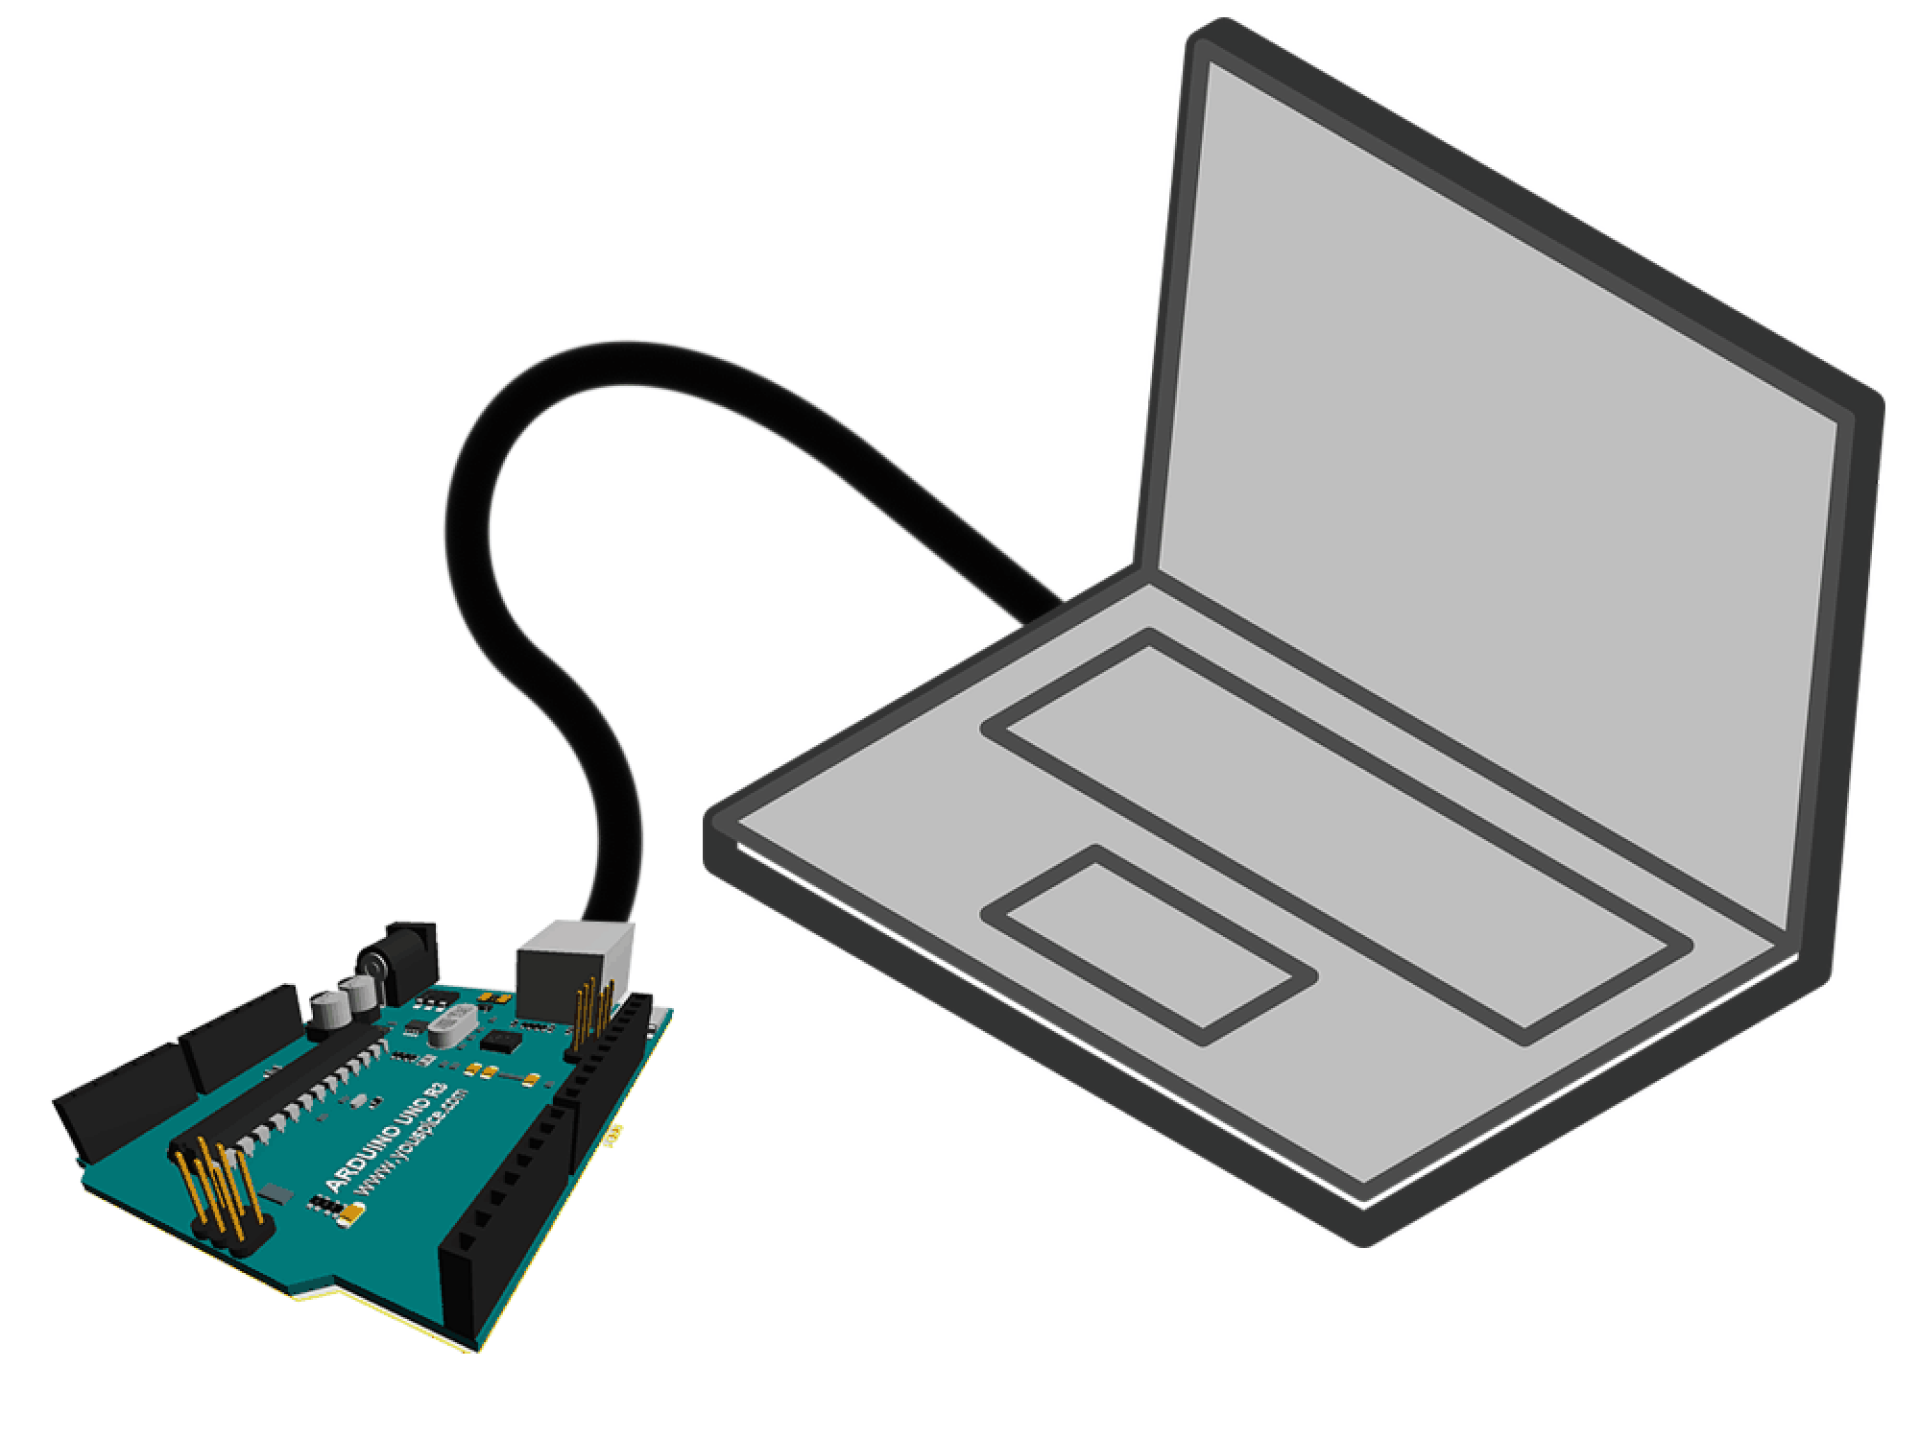
\includegraphics[width=0.8\linewidth]{P2/img/per1/step 1.png}
			\caption{Step 1}
			\label{fig:Step 1(Step 1)}
		\end{figure}
		\item Buka software Arduino IDE, lalu pilih new sketch.
		\begin{figure}[H]
			\centering
			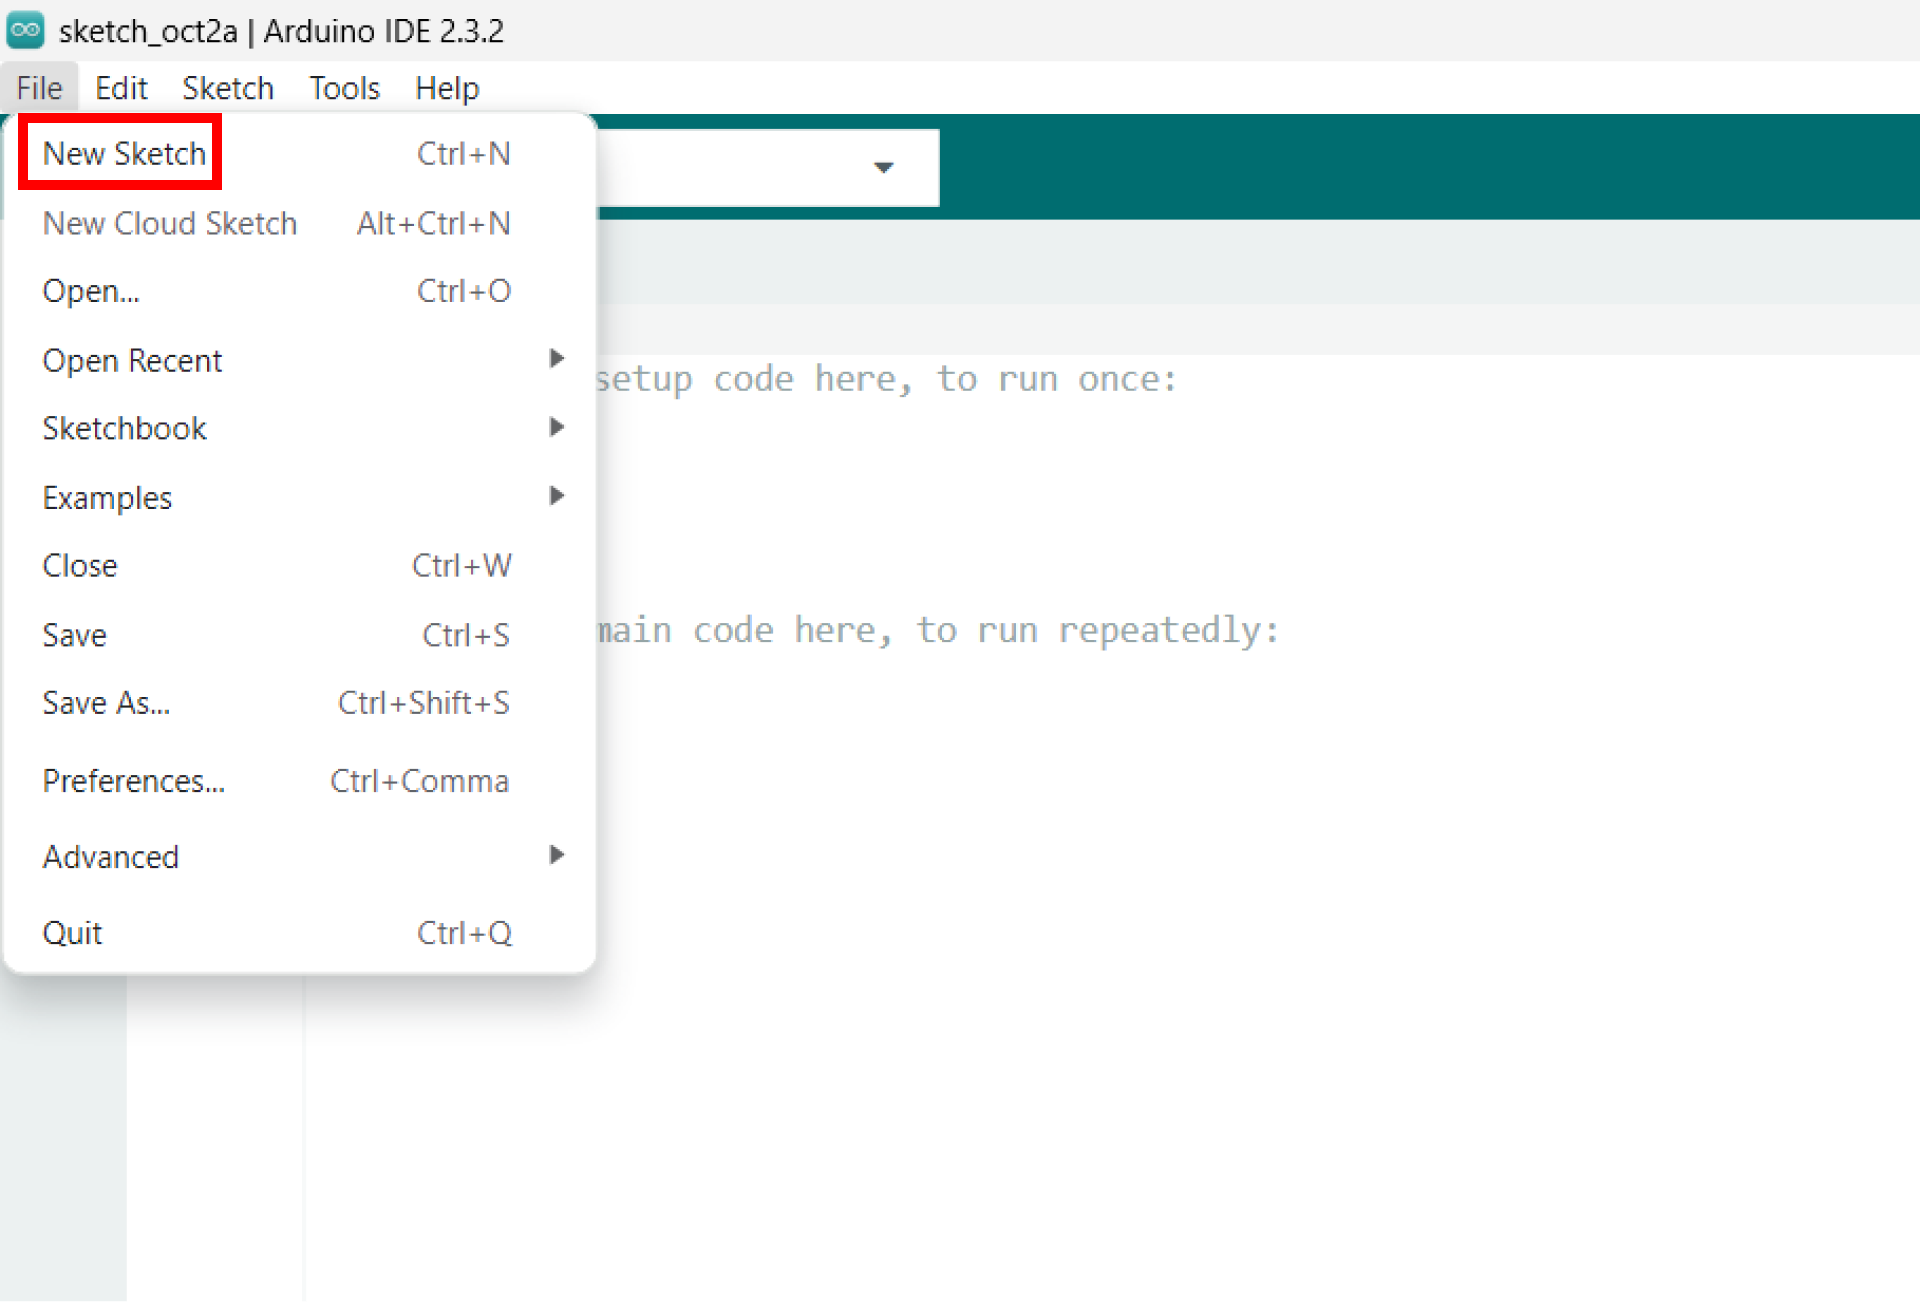
\includegraphics[width=0.8\linewidth]{P2/img/per1/step 2.png}
			\caption{Step 2}
			\label{fig:Step 2(Step 2)}
		\end{figure}
		\item Buka menu Tools, lalu cek Board dan Port yang terhubung apakah sudah benar
		\\(Port bergantung pada device, jadi bisa berbeda dengan port di Modul).
		\begin{figure}[H]
			\centering
			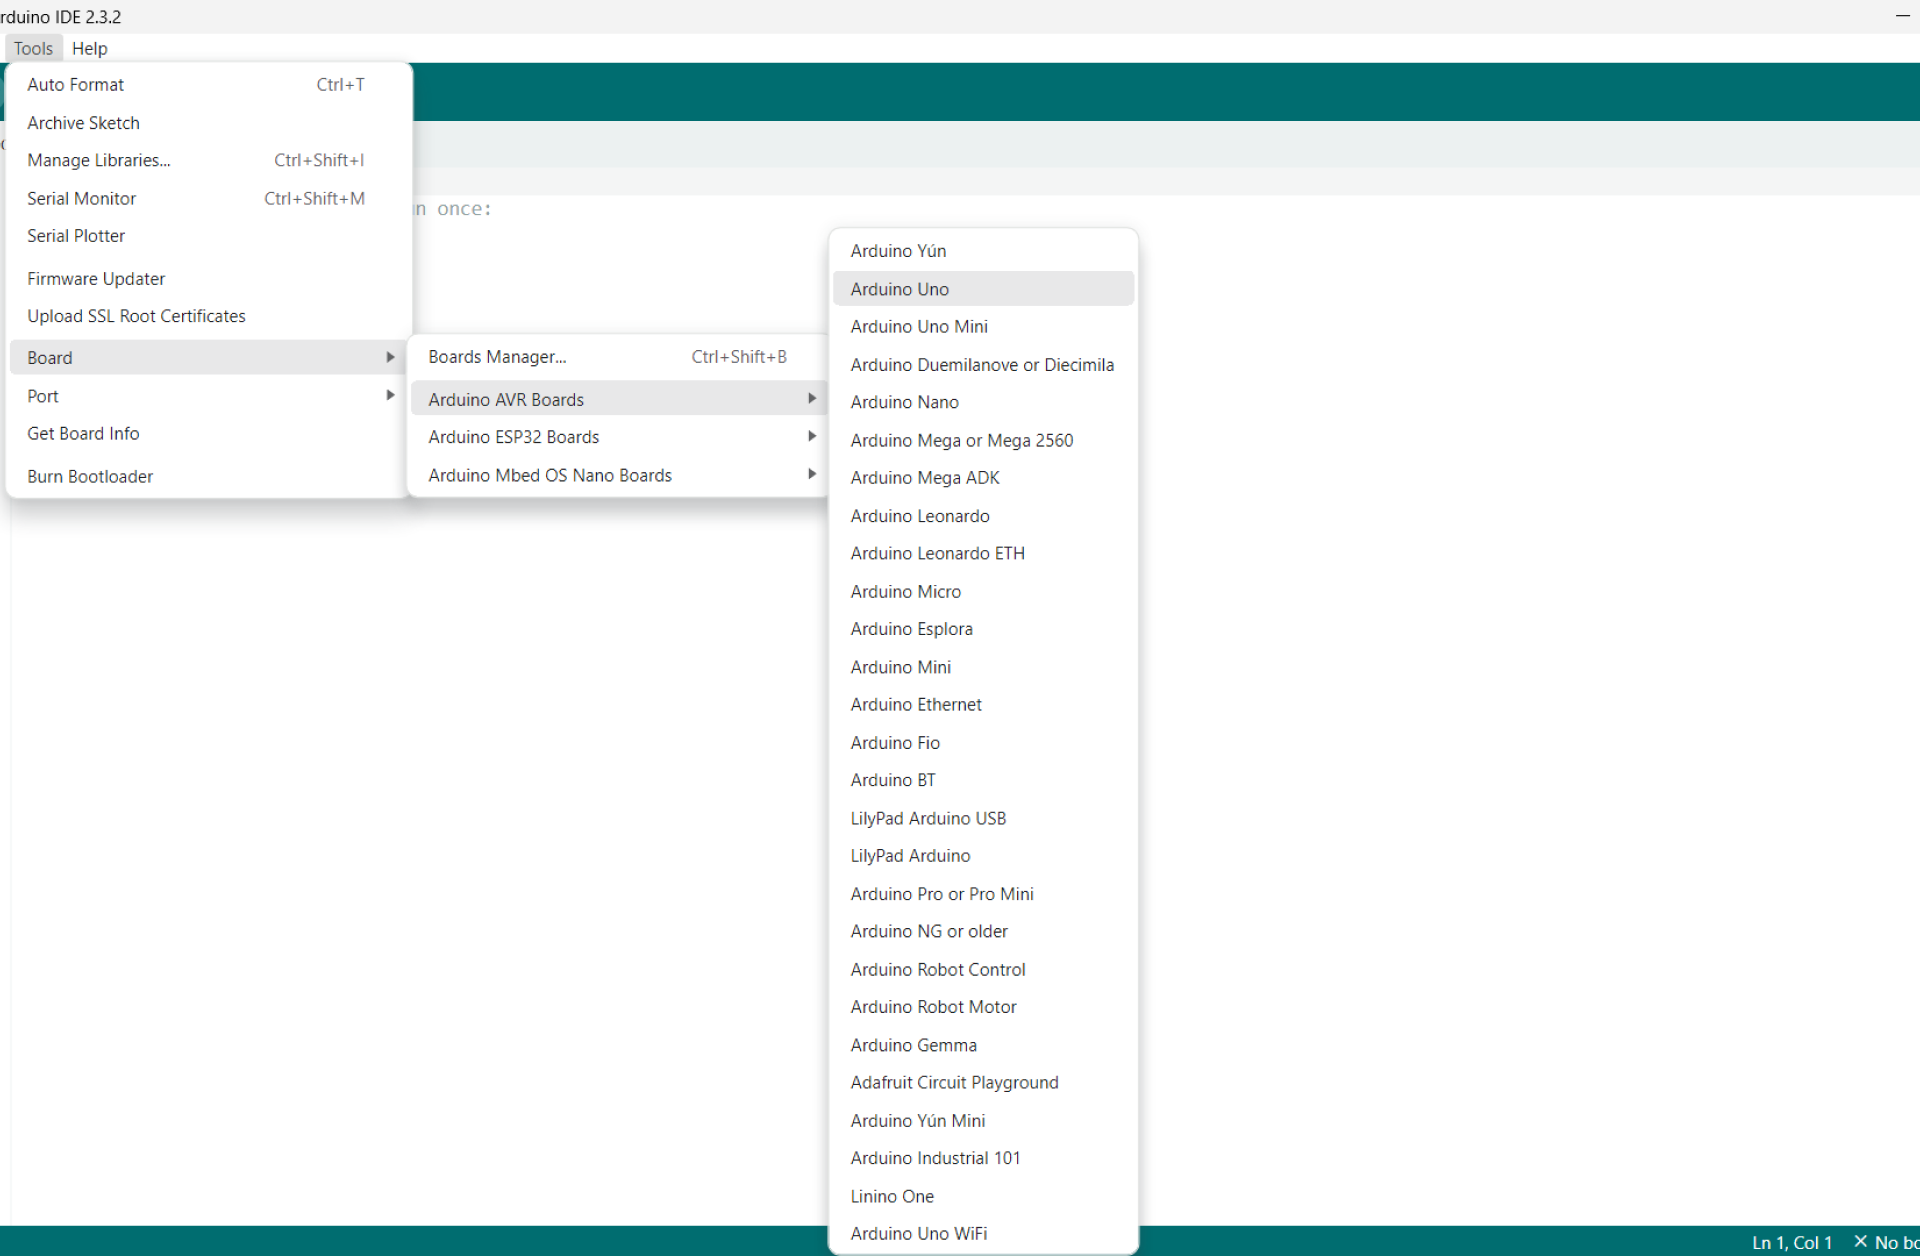
\includegraphics[width=0.8\linewidth]{P2/img/per1/step 3.png}
			\caption{Step 3}
			\label{fig:Step 3(Step 3)}
		\end{figure}

		\begin{figure}[H]
			\centering
			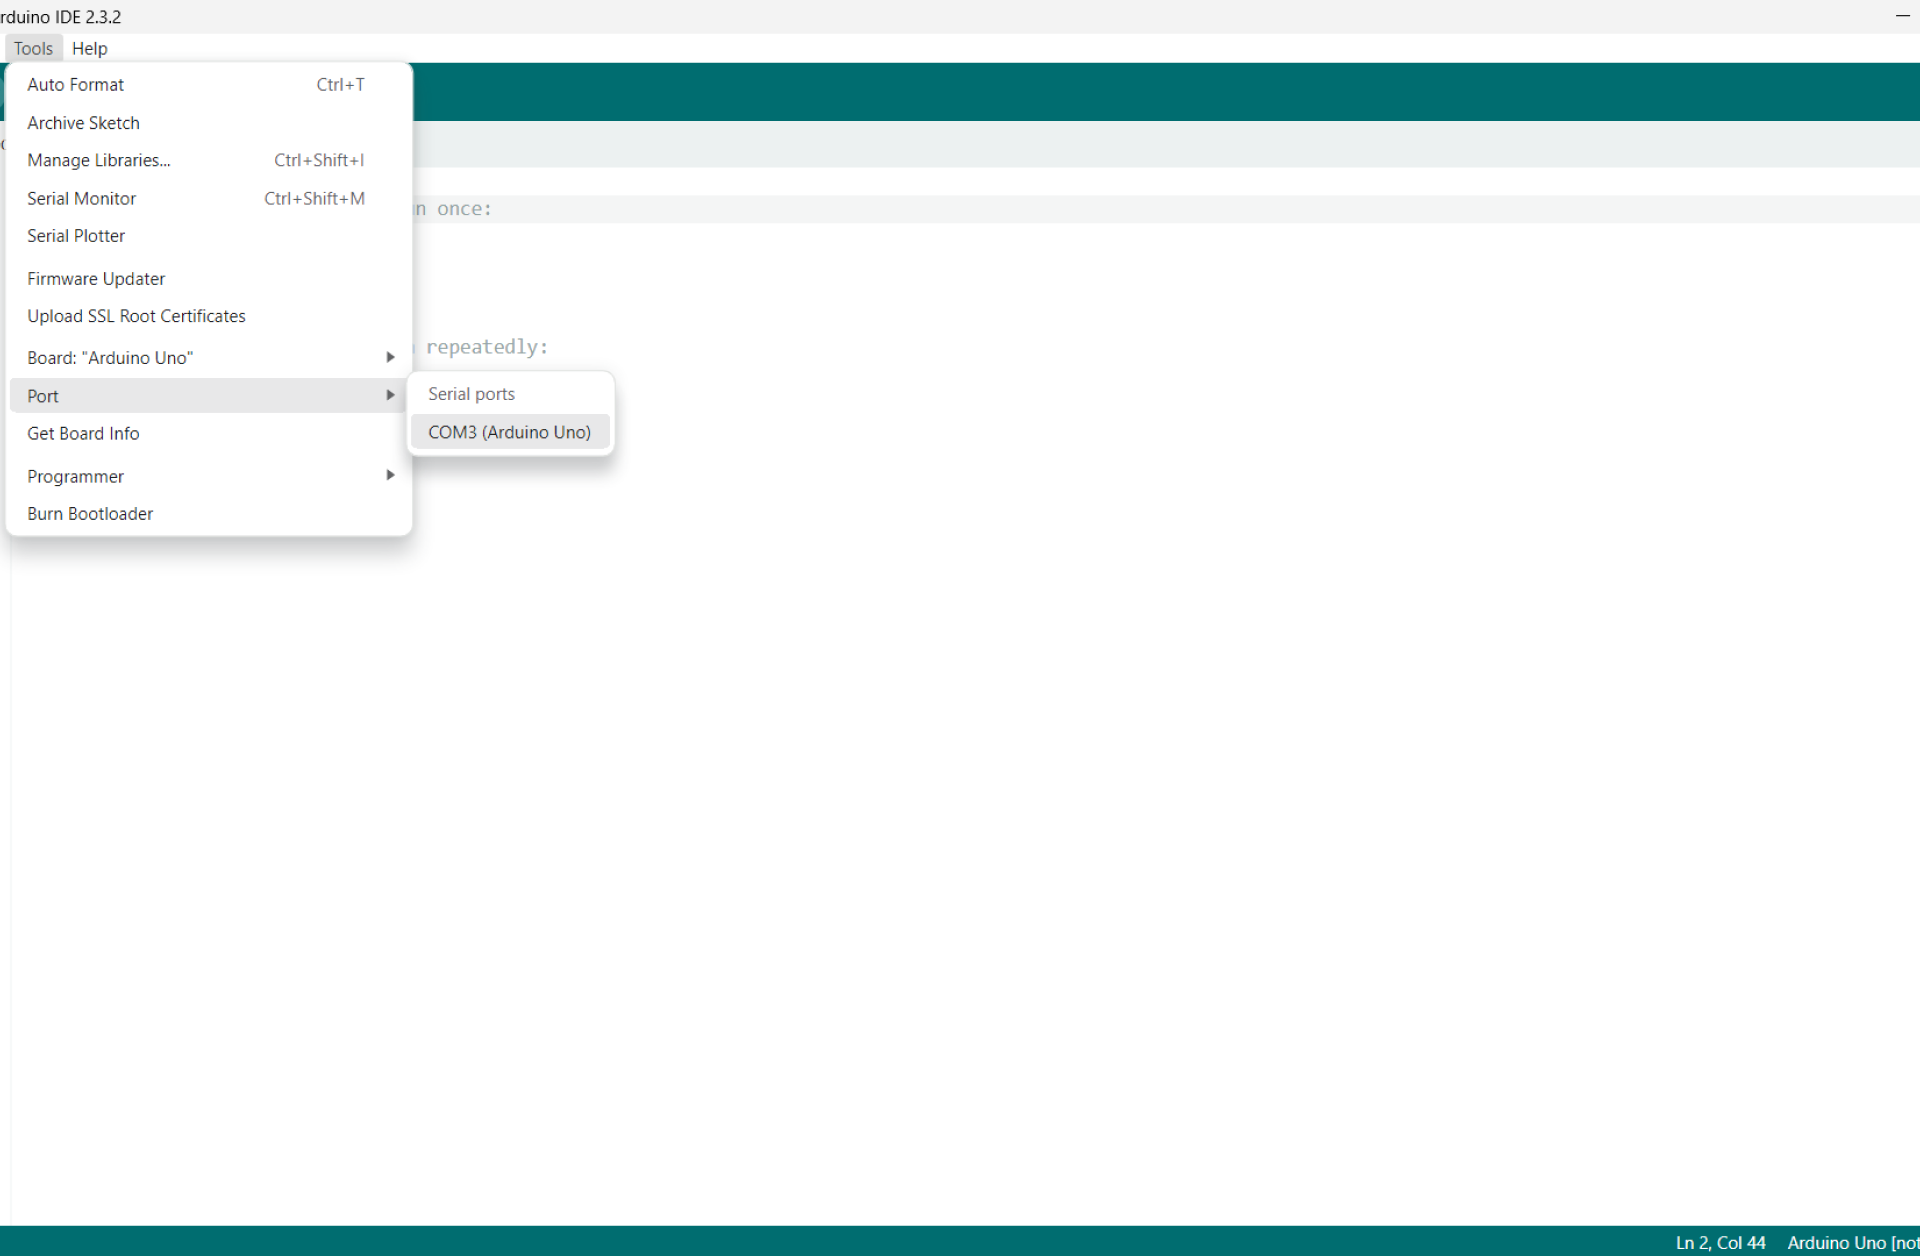
\includegraphics[width=0.8\linewidth]{P2/img/per1/step 4.png}
			\caption{Step 4}
			\label{fig:Step 4(Step 4)}
		\end{figure}

	\end{enumerate}

	\textbf{Kode Program Arduino}
	\begin{enumerate}
		\item Masukkan kode program dibawah ini untuk menjalankan ADC (Analog to Digital Converter) pada Arduino IDE.
		\begin{figure}[H]
			\centering
			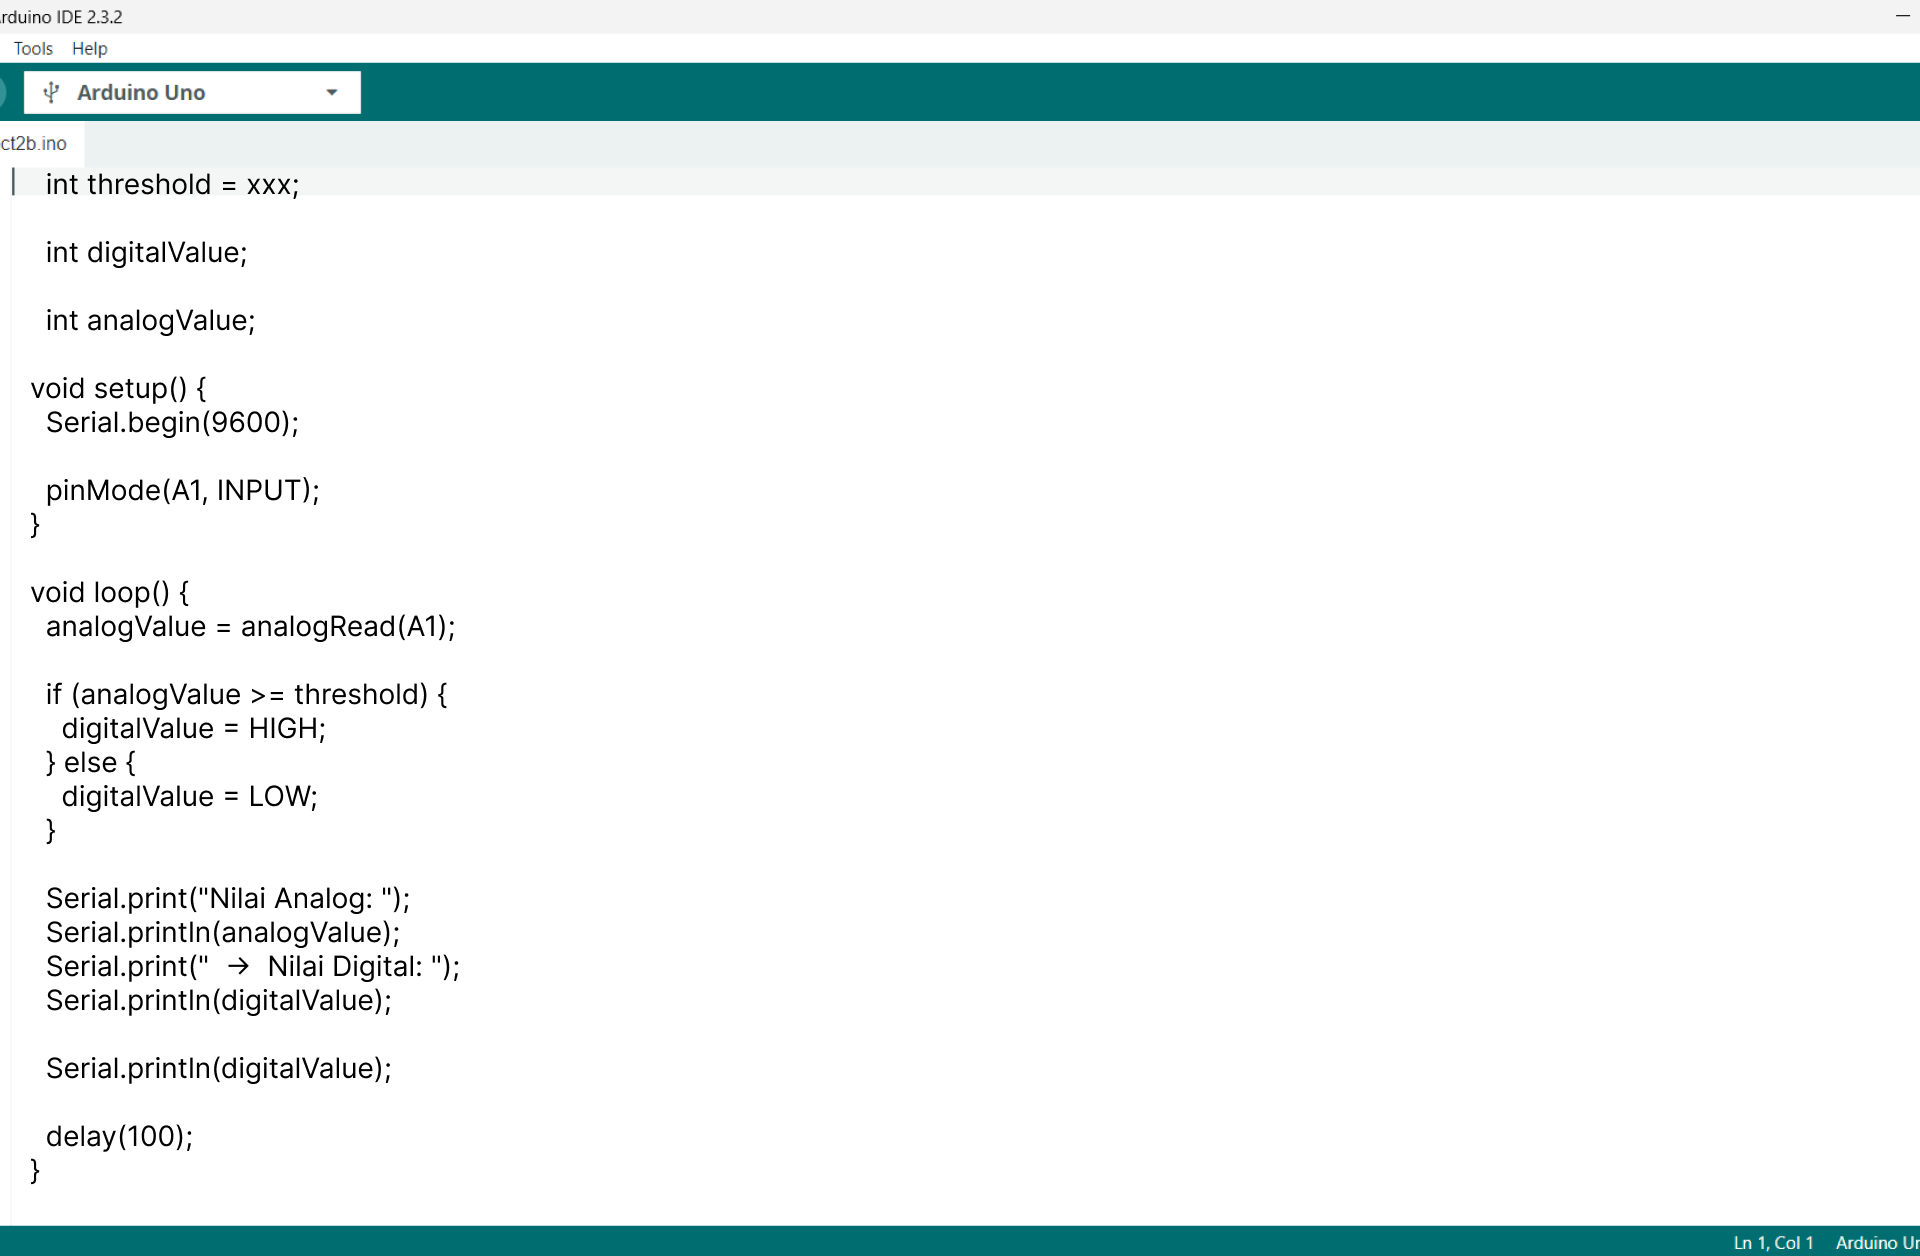
\includegraphics[width=0.8\linewidth]{P2/img/per1/step 5.png}
			\caption{Step 5}
			\label{fig:Step 5(Step 5)}
		\end{figure}

		\item Klik verify, apabila berhasil maka klik upload.
		\begin{figure}[H]
			\centering
			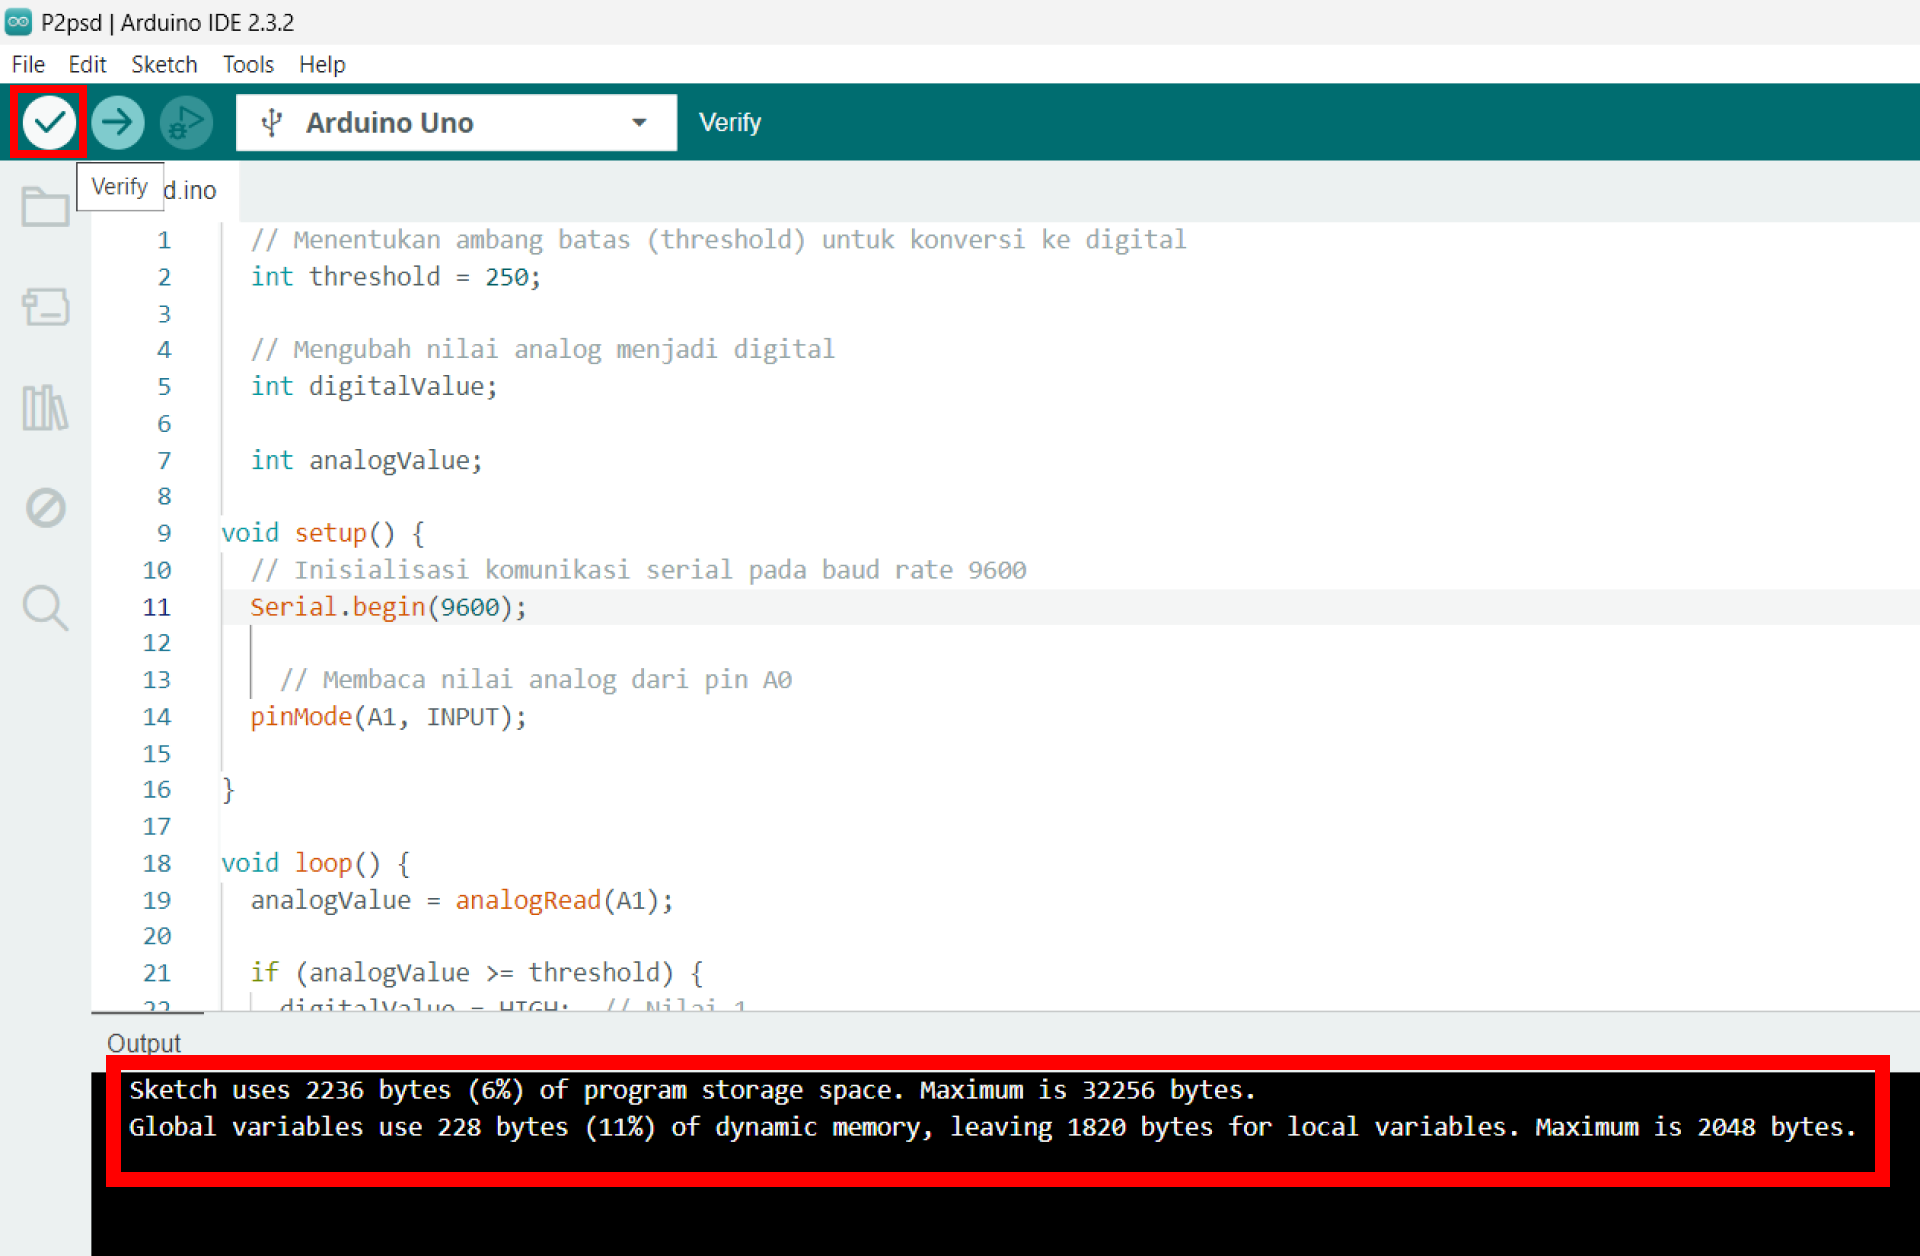
\includegraphics[width=0.8\linewidth]{P2/img/per1/step 6.png}
			\caption{Step 6}
			\label{fig:Step 6(Step 6)} 
		\end{figure}

		\item Klik upload, bisa terlihat done uploading di pojok kanan bawah. 
		\begin{figure}[H]
			\centering
			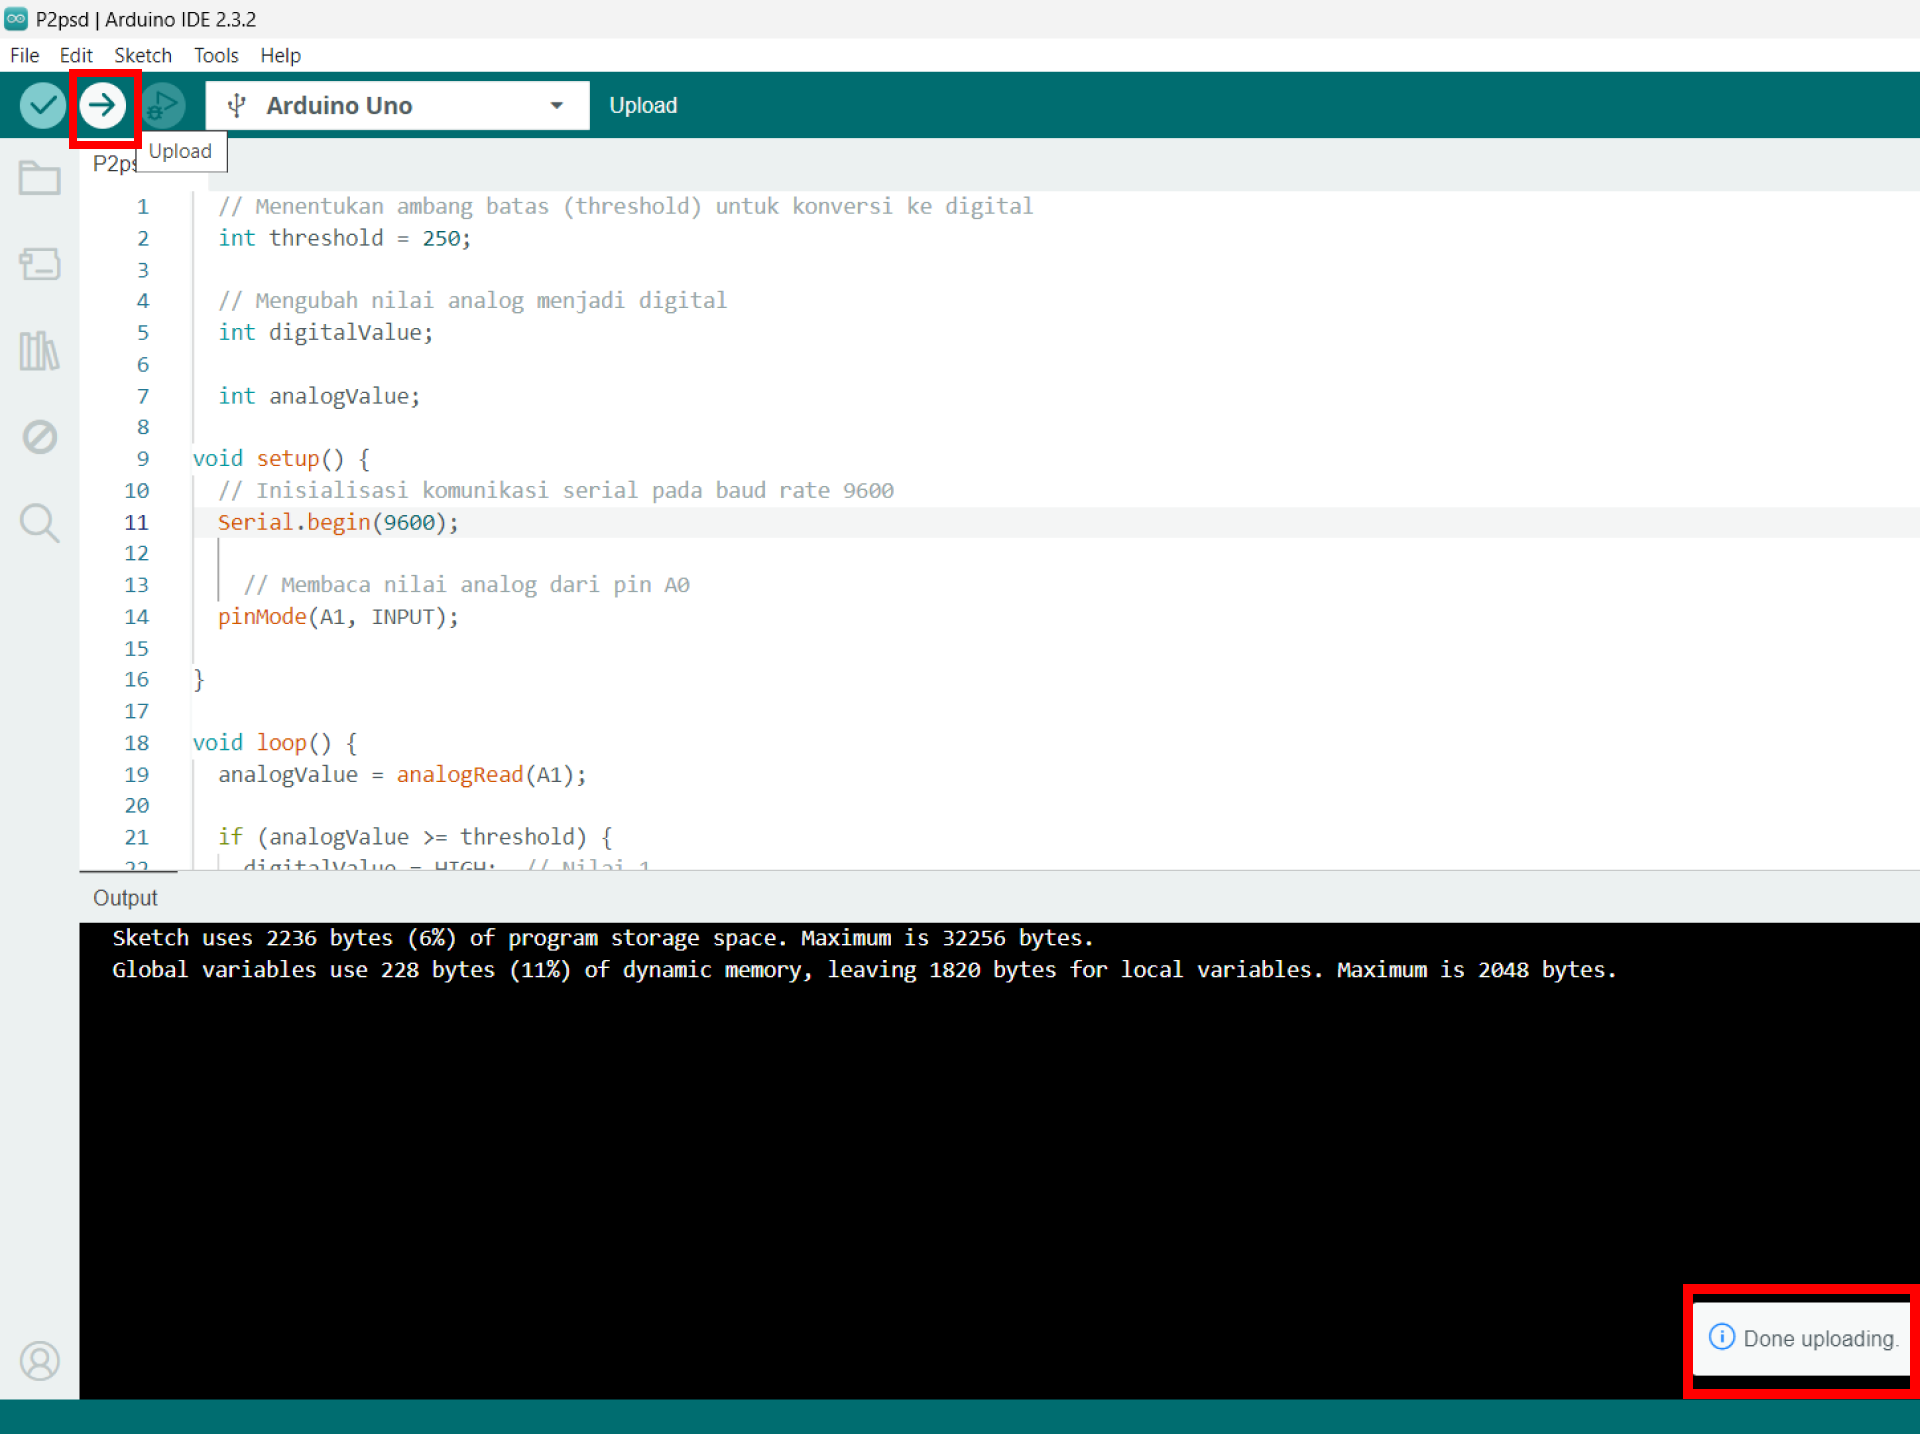
\includegraphics[width=0.8\linewidth]{P2/img/per1/step 7.png}
			\caption{Step 7}
			\label{fig:Step 7(Step 7)} 
		\end{figure}
	\end{enumerate}

	\textbf{Memulai Function Generator}
	\begin{enumerate}
		\item Klik tombol power, untuk menyalakan function generator.
		\begin{figure}[H]
			\centering
			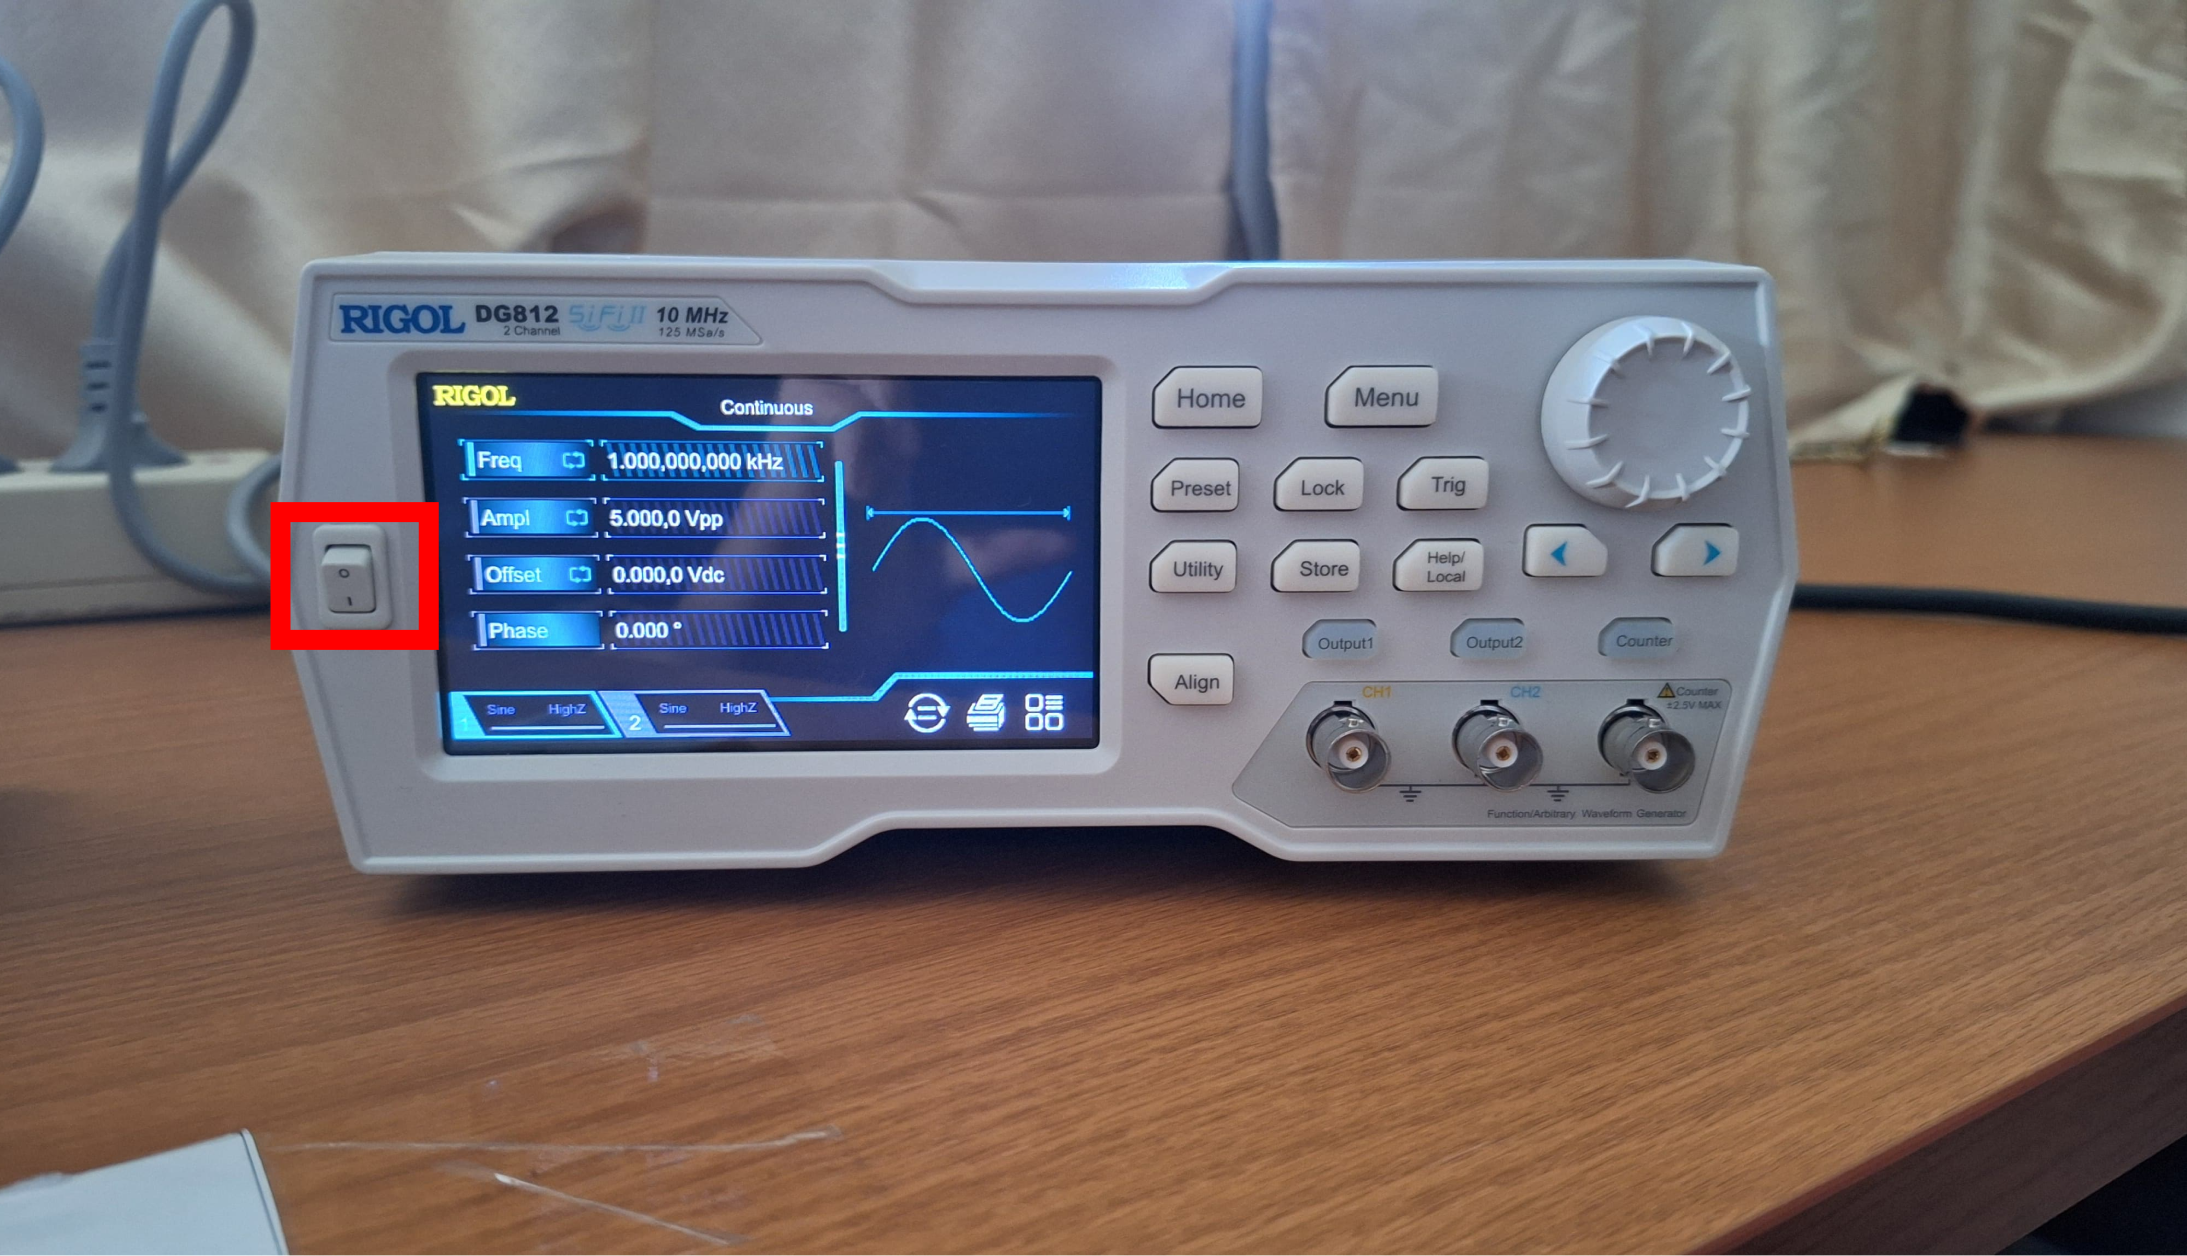
\includegraphics[width=0.8\linewidth]{P2/img/per1/step 8.png}
			\caption{Step 8}
			\label{fig:Step 8(Step 8)}
		\end{figure}

		\item Konfigurasi sinyal input pada Function generator.
		\begin{figure}[H]
			\centering
			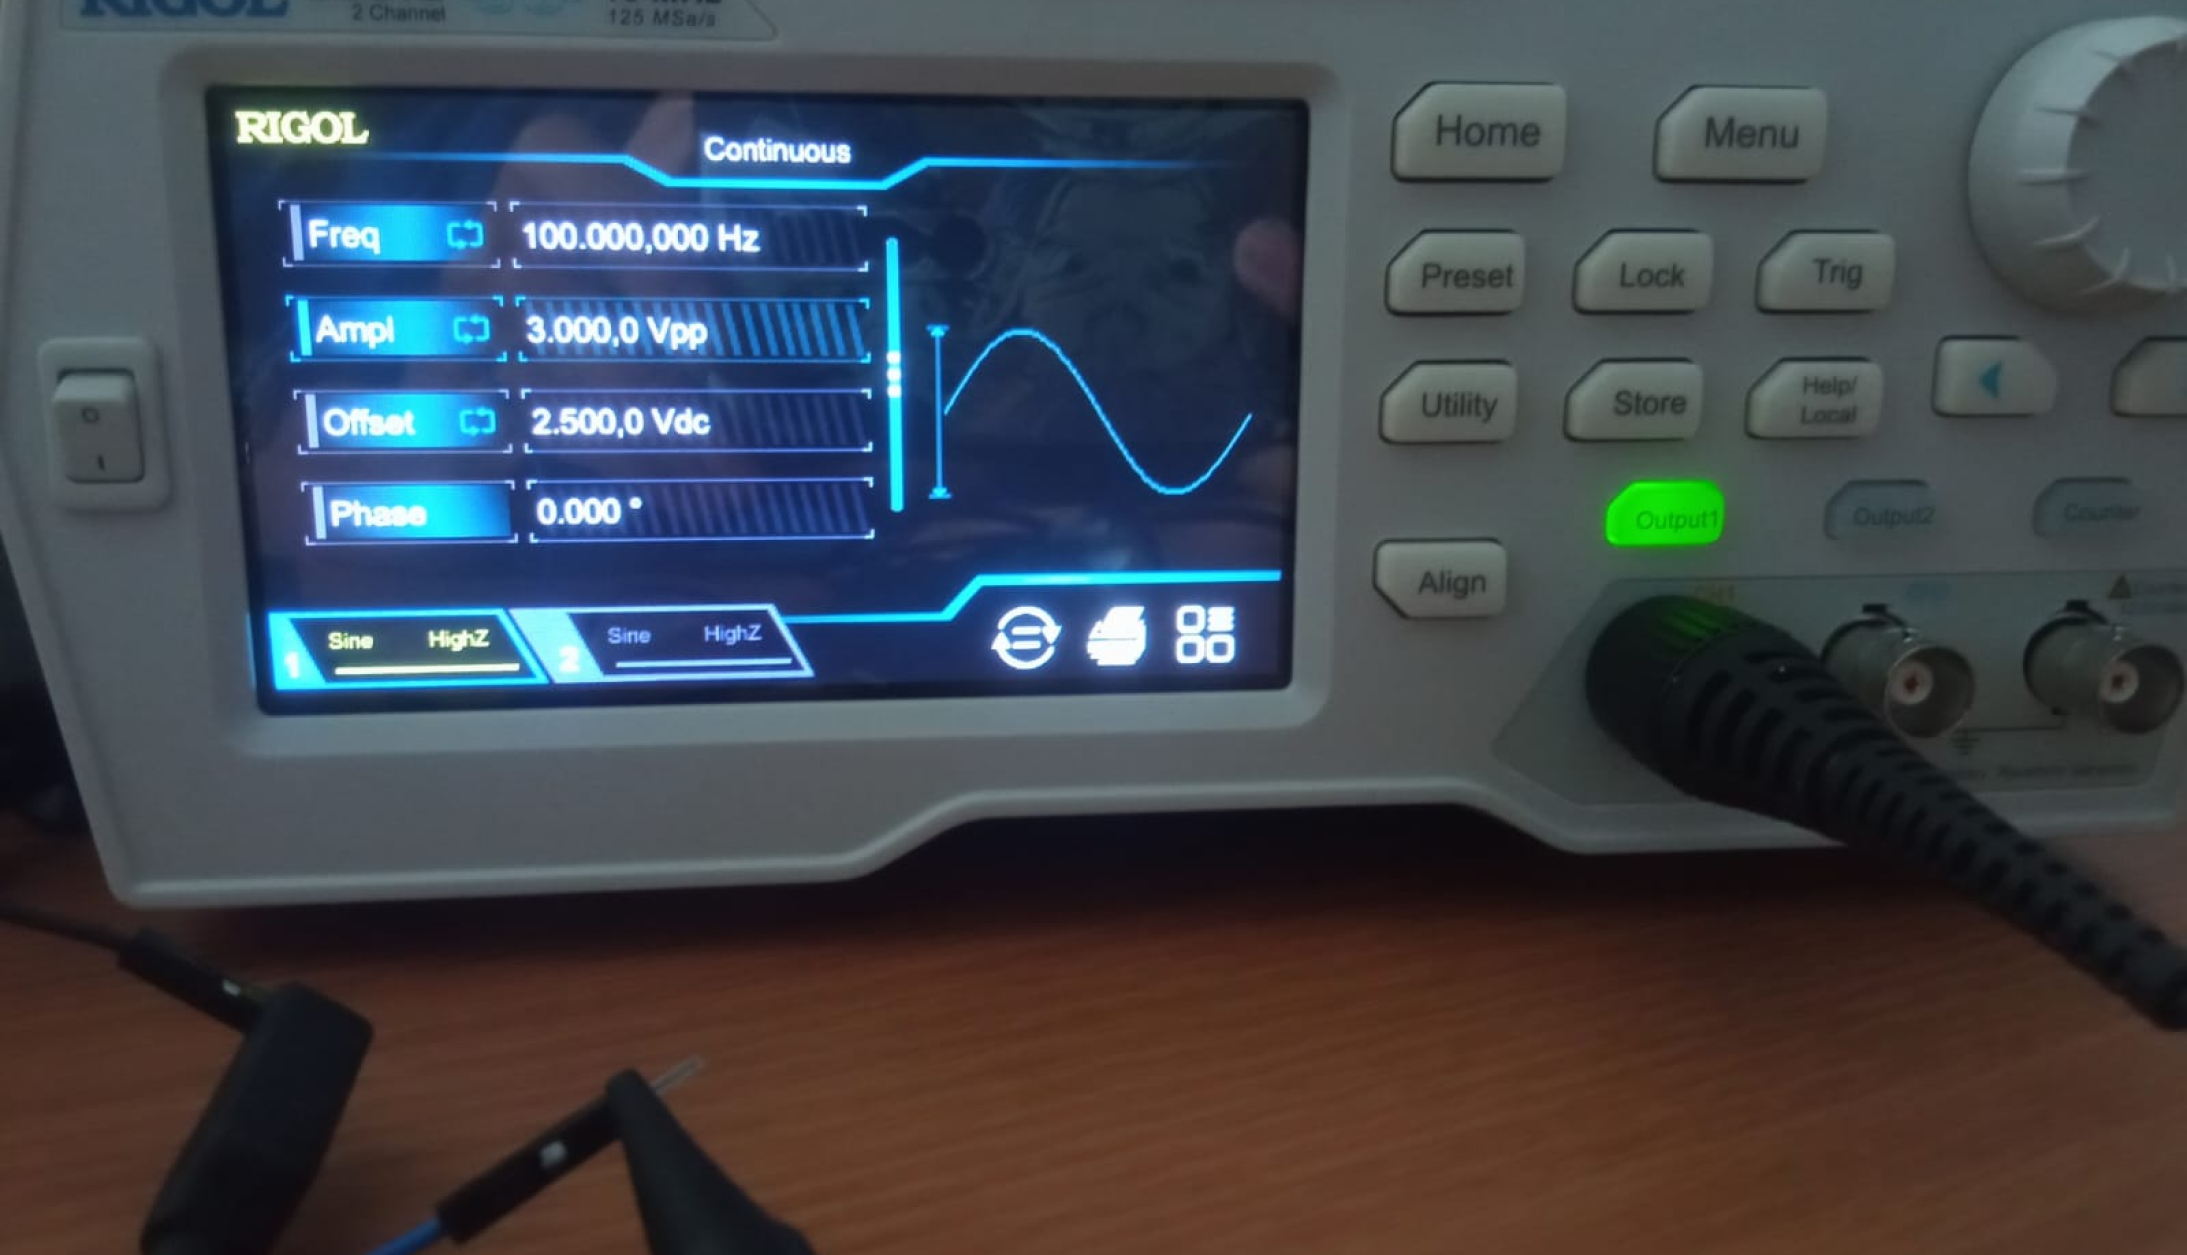
\includegraphics[width=0.8\linewidth]{P2/img/per1/step 9.png}
			\caption{Step 9}
			\label{fig:Step 9(Step 9)}
		\end{figure}
	\end{enumerate}

	\textbf{Konfigurasi Arduino}
	\begin{enumerate}
		\item Hubungkan kabel jumper ke salah satu pin Analog Arduino, kemudian hubungan ke probe.
		\\pengait (positif) Function generator.
		\begin{figure}[H]
			\centering
			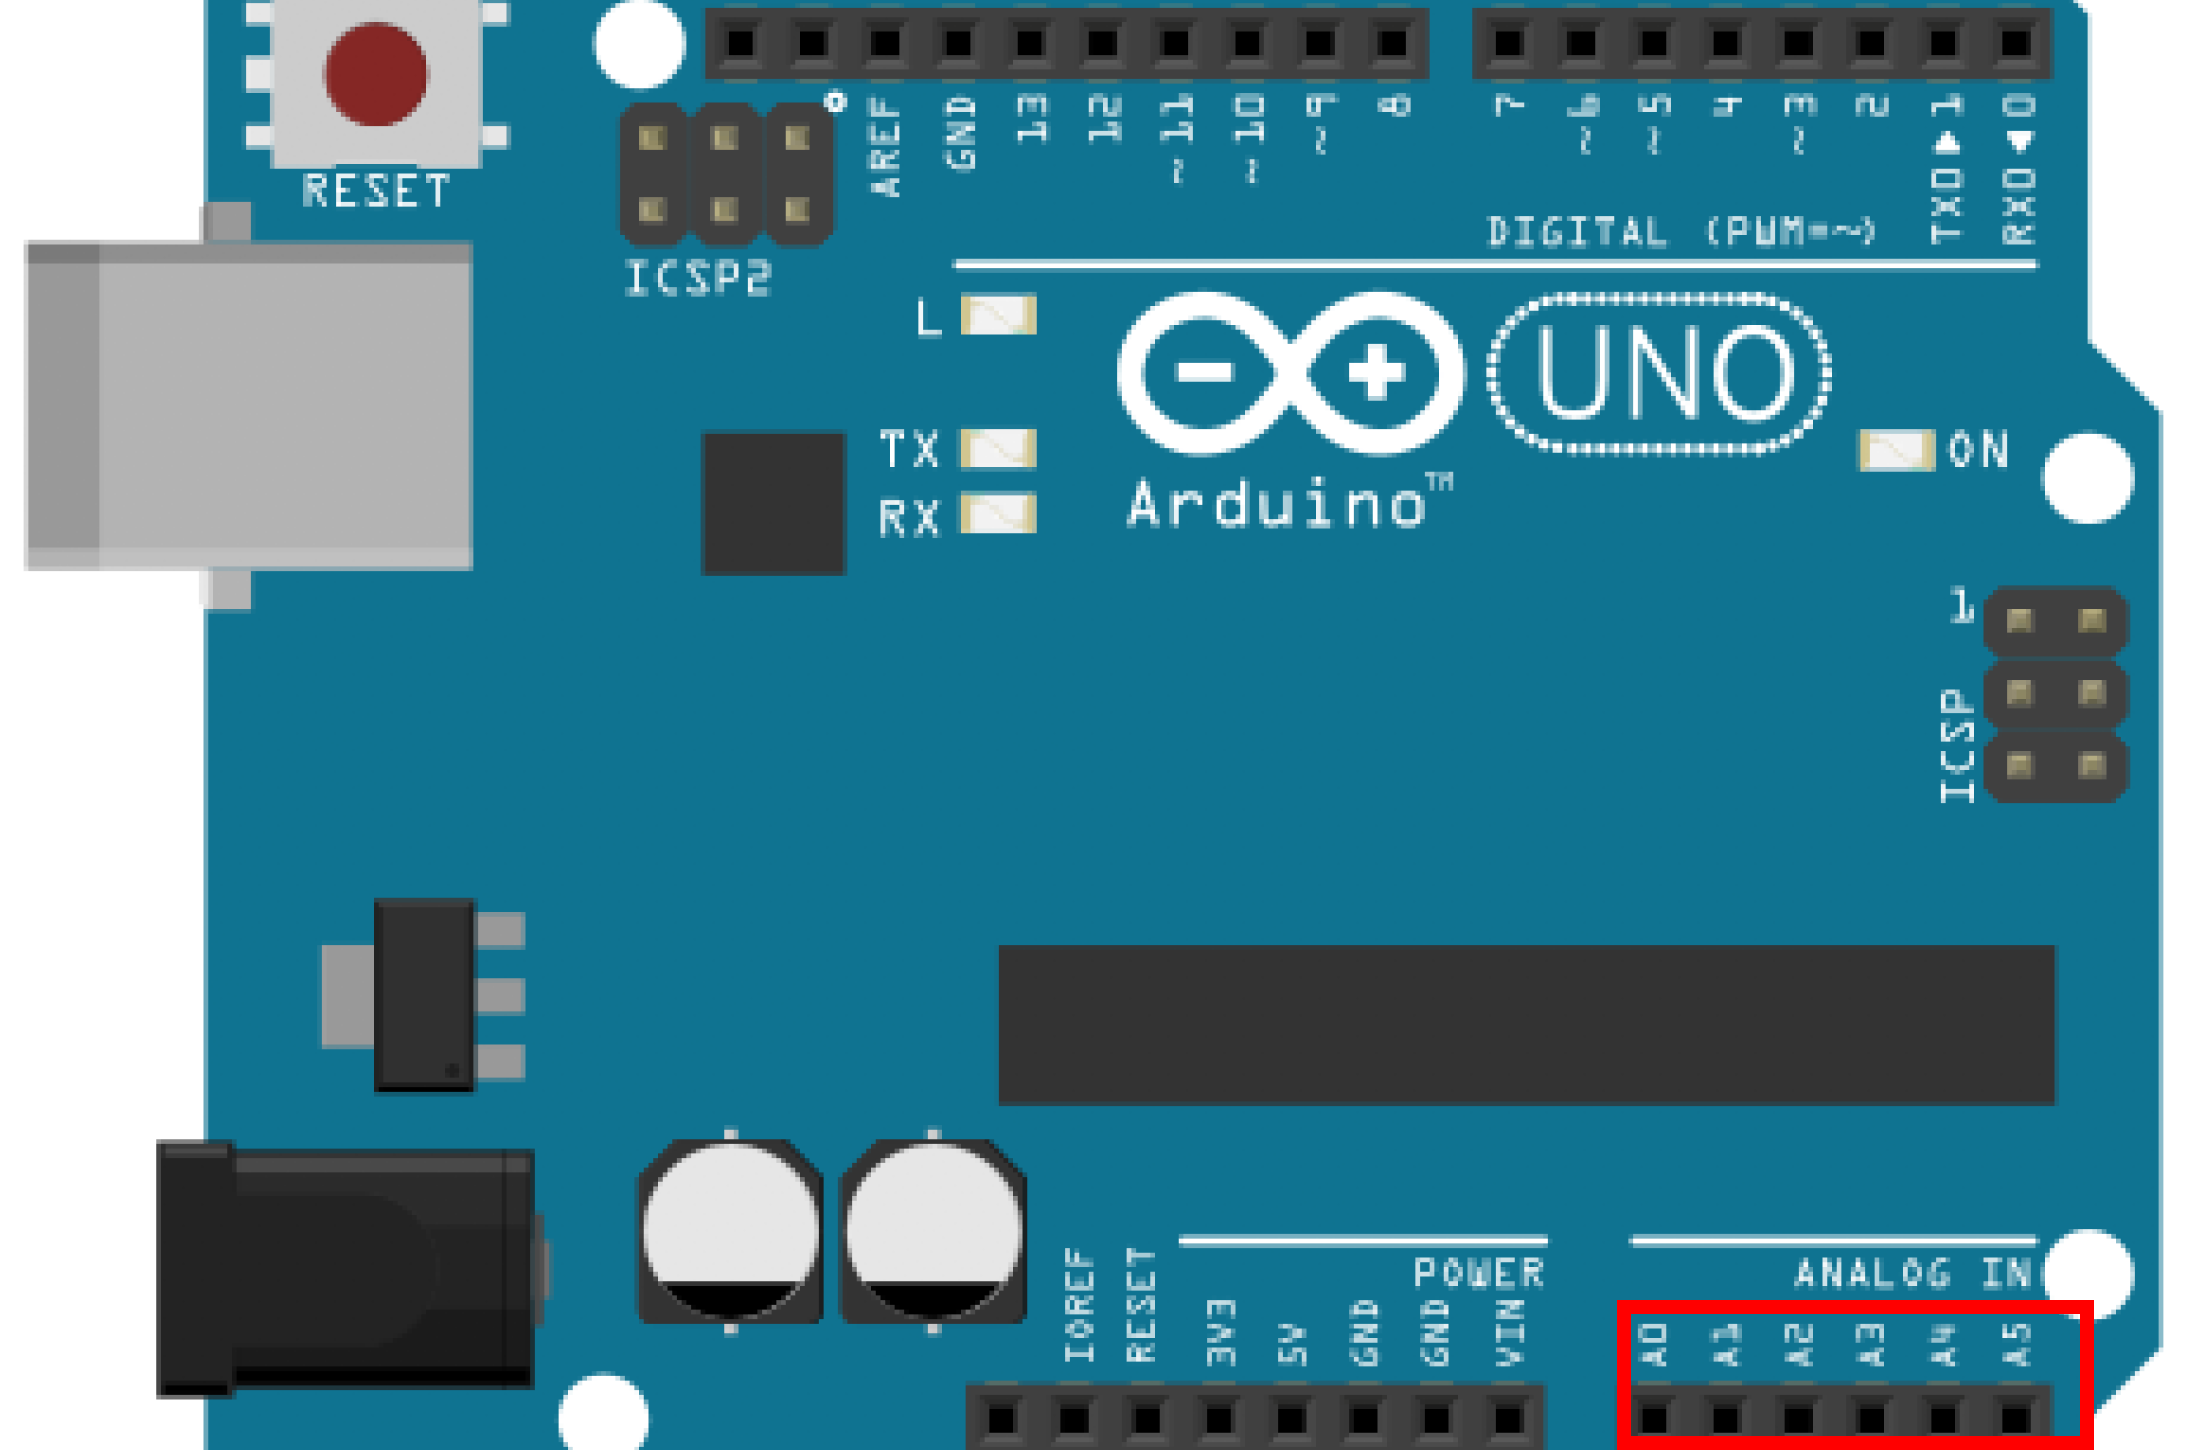
\includegraphics[width=0.8\linewidth]{P2/img/per1/step 10.png}
			\caption{Step 10}
			\label{fig:Step 8(Step 10)}
		\end{figure}

		\item Hubungkan kabel jumper ke salah satu pin GND Arduino, kemudian hubungkan probe.
		\\penjepit buaya (negatif) Function generator.
		\begin{figure}[H]
			\centering
			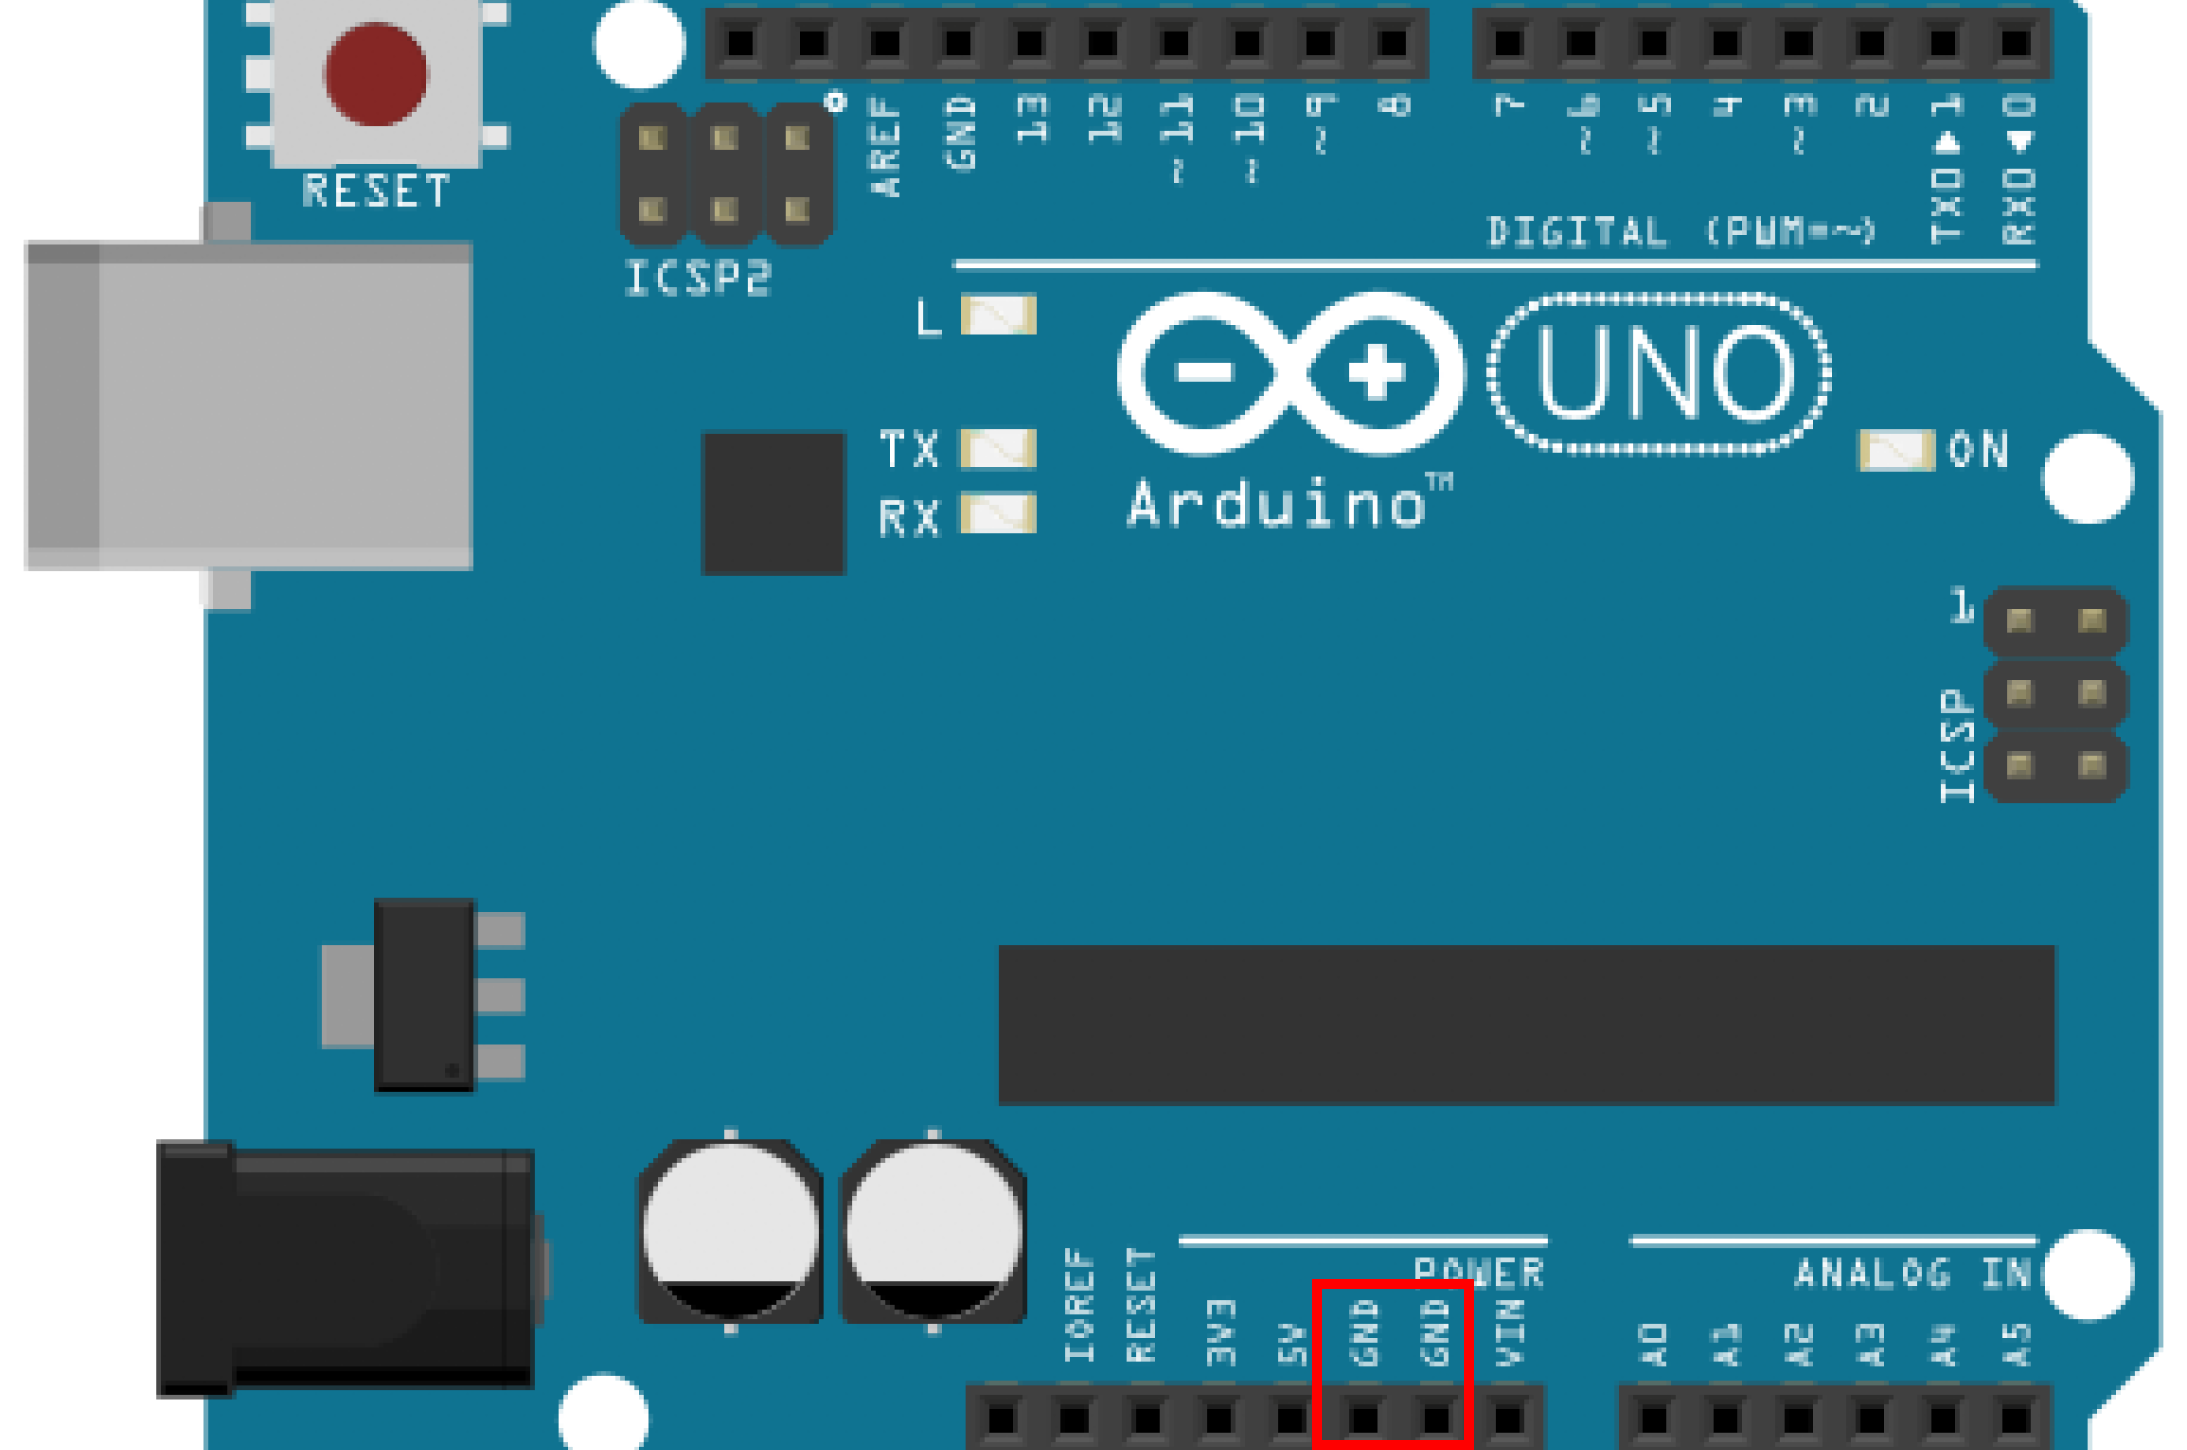
\includegraphics[width=0.8\linewidth]{P2/img/per1/step 11.png}
			\caption{Step 11}
			\label{fig:Step 11(Step 11)}
		\end{figure}

		\item Nyalakan Output 1 pada Function Generator.
		\item Buka Serial plotter di pojok kanan atas pada Arduino IDE.
		\item Buka Serial Monitor di pojok kanan atas pada Arduino IDE.
	\end{enumerate}

\end{center}

%======================PERCOBAAN 2==========================%
\subsection{Percobaan 2}
\begin{center}
	\textbf{Konfigurasi Osiloskop}
	\begin{enumerate}
		\item Hubungkan kabel power ke osiloskop, lalu tekan tombol power untuk menyalakan Osiloskop. 
		\begin{figure}[H]
			\centering
			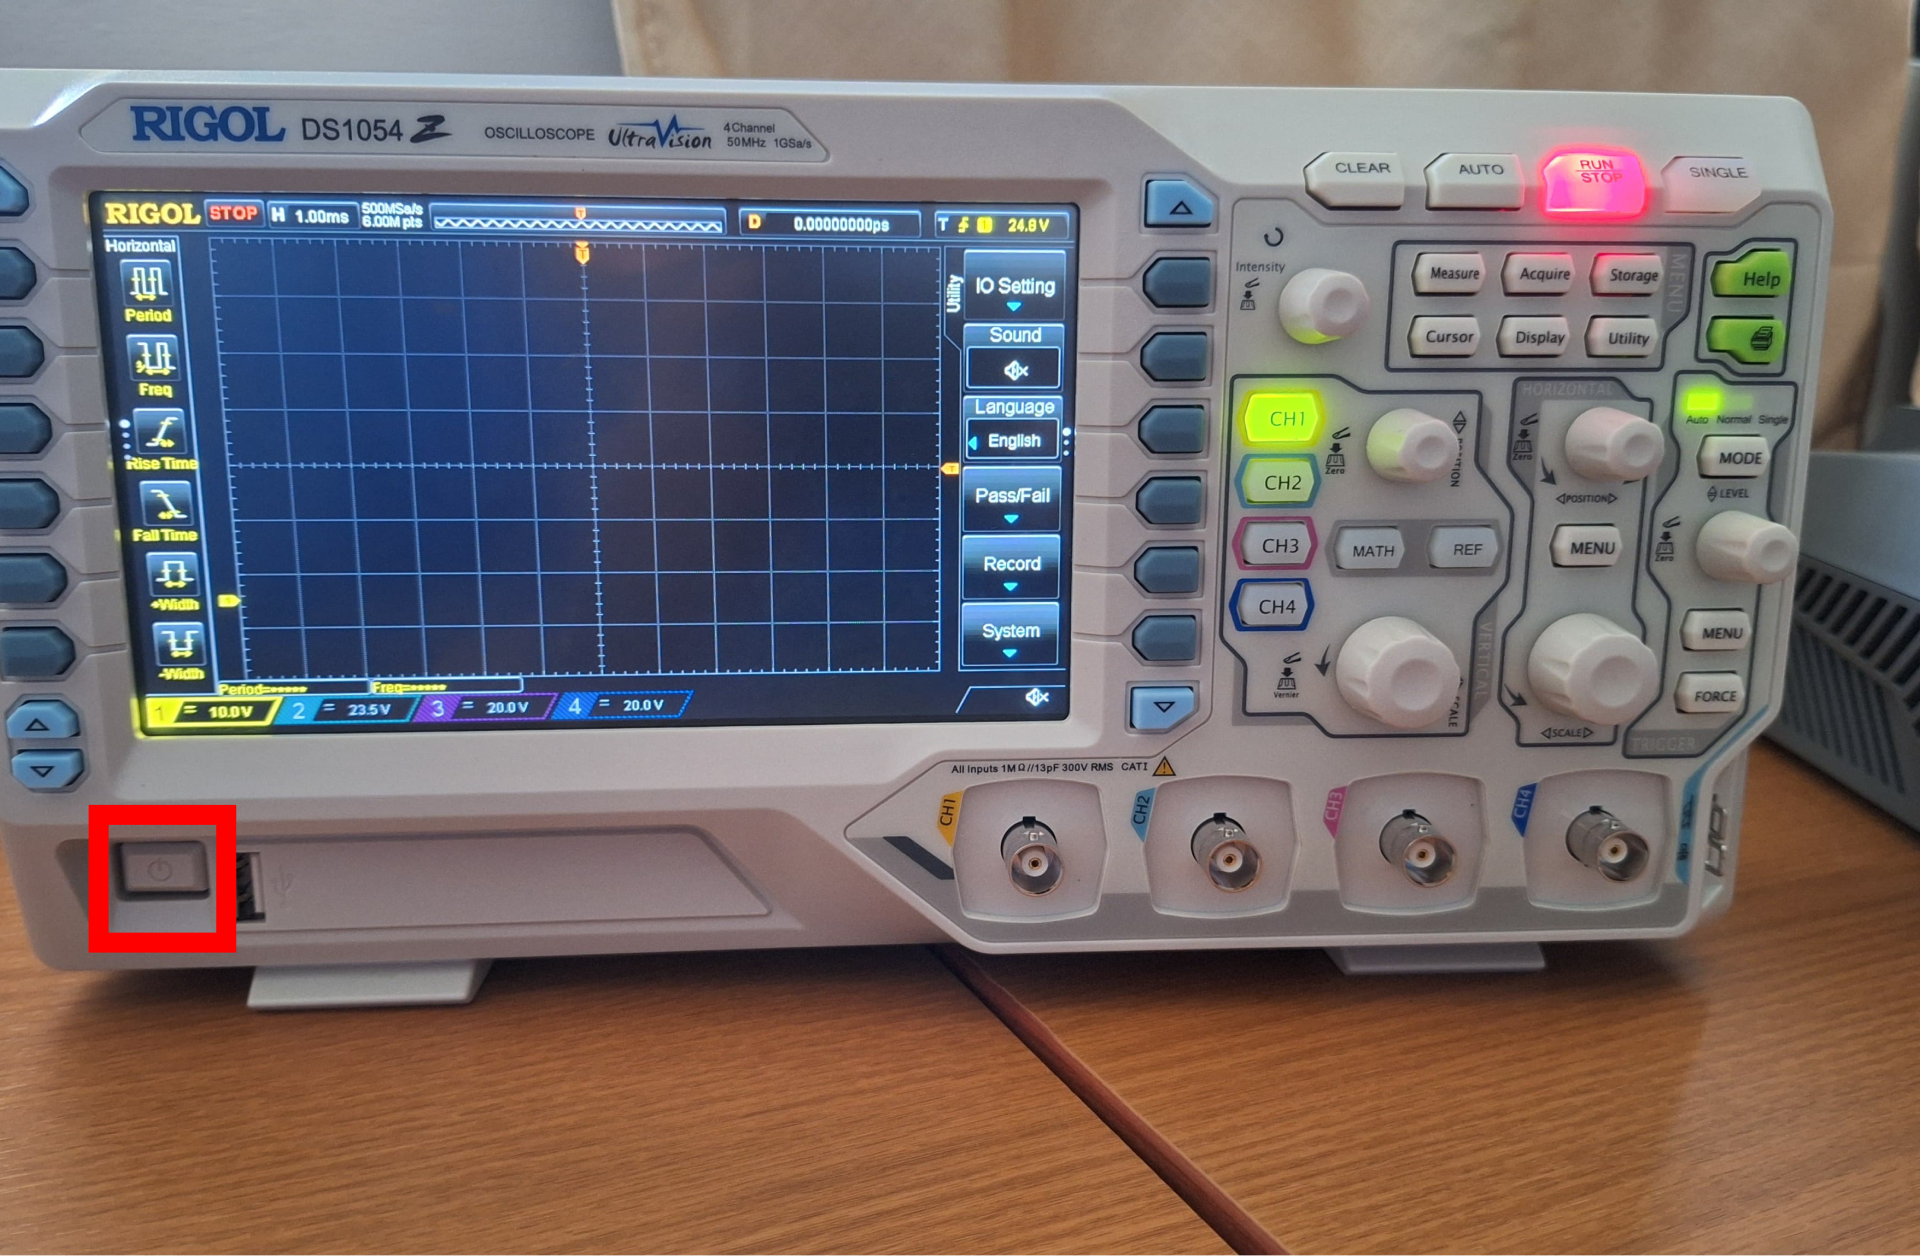
\includegraphics[width=0.9\linewidth]{P2/img/per2/step 1.png}
			\caption{Step 1}
			\label{fig:Step 1(Step 1)}
		\end{figure}
		\item Hubungkan kabel probe pada channel 1. 
		\begin{figure}[H]
			\centering
			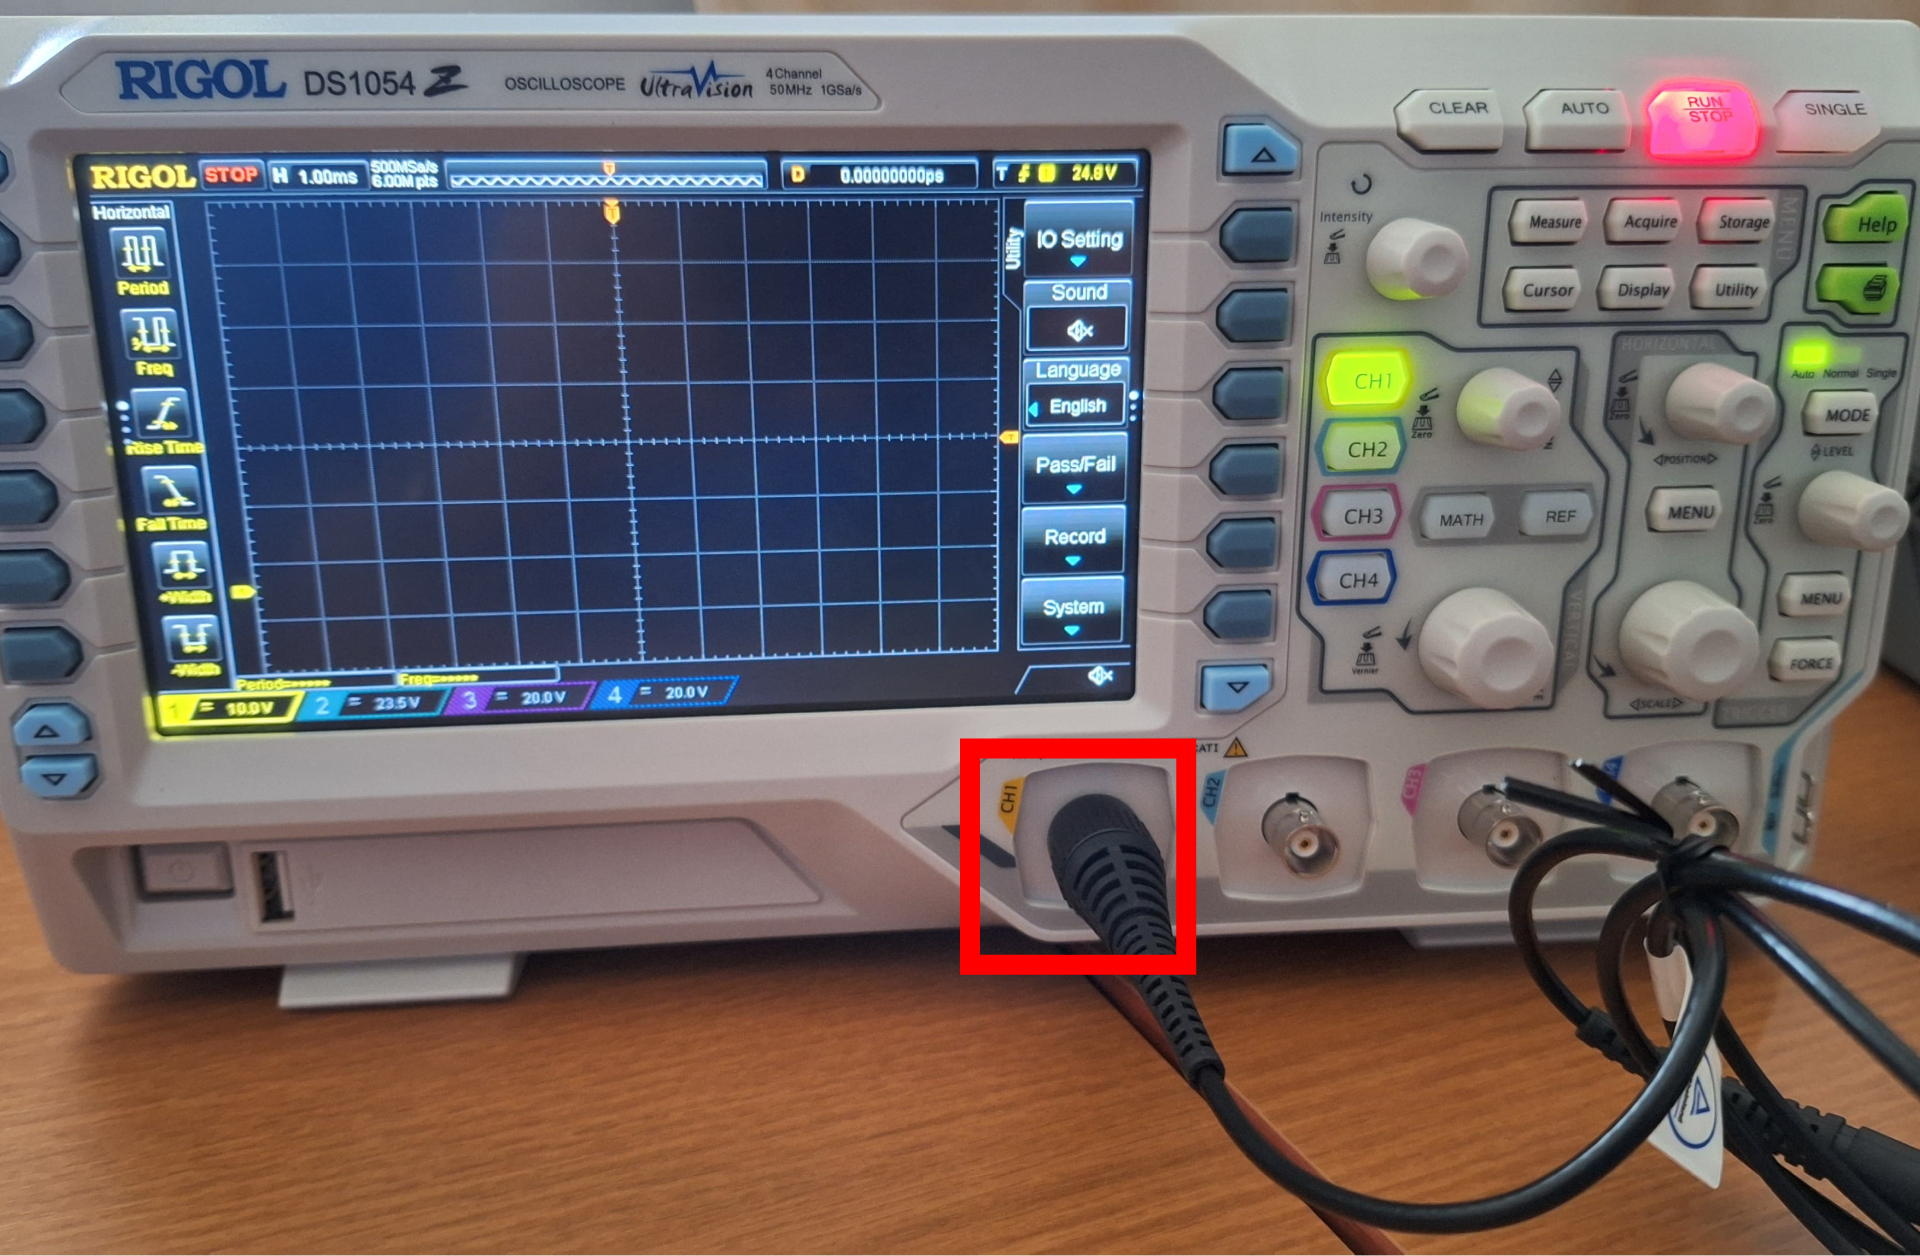
\includegraphics[width=0.8\linewidth]{P2/img/per2/step 2.png}
			\caption{Step 2}
			\label{fig:Step 2(Step 2)}
		\end{figure}
		\item Hubungkan kabel jumper dari salah satu pin Analog Arduino dengan probe pengait (positif) osiloskop dan function generator.
		\item Hubungkan kabel jumper pin GND Arduino dengan probe penjepit buaya (negatif) osiloskop.
		\item Klik AUTO pada Osiloskop.
		\item Bandingkan hasil sinyal yang ditampilkan oleh Serial plotter Arduino dengan Osiloskop.
	\end{enumerate}	
\end{center}

%===========================================================%
\section{Hasil yang didapat}
Memahami perbedaan hasil sinyal digital yang diperoleh oleh Arduino dan Osiloskop.

%===========================================================%
\section{Kesimpulan}
Mengetahui hasil sinyal manakah yang lebih baik dihasilkan dari kedua perangkat \\Arduino dan Osiloskop. 


